\documentclass[graybox]{svmult}
\usepackage[hyperfootnotes=false]{hyperref}
\hypersetup{bookmarksdepth=3}

\usepackage{mathptmx}       \usepackage{helvet}         \usepackage{courier}        \usepackage{type1cm}                                    \usepackage{makeidx}         \usepackage{graphicx}                                     \usepackage{multicol}        \usepackage[bottom]{footmisc} \usepackage{adjustbox}
 \usepackage{multirow}
 \usepackage{algorithm}
 \usepackage{algpseudocode}
 \usepackage{ifthen}
 \usepackage{csquotes}
 \usepackage{amsmath}

\usepackage{comment}
 \usepackage{natbib}
 \setcitestyle{numbers,square}
 \usepackage[subrefformat=parens,labelformat=simple,caption=false,labelfont={bf}]{subfig}
 \usepackage[nolist,smaller]{acronym}
\allowdisplaybreaks
\makeindex

\begin{document}
\begin{acronym}[ALSPAC]
  \acro{FAS}{Foetal Alcohol Syndrome}
  \acro{CPT}{Cumulative Prospect Theory}
  \acro{PT}{Prospect Theory}
  \acro{NICE}{the National Institute for Health and Care Excellence}
  \acro{IAPT}{Improving Access to Psychological Therapies}
  \acro{CMACE}{Centre for Maternal and Child Enquiries}
  \acroindefinite{CMACE}{the}{the}
  \acro{AUDIT}{Alcohol Use Disorders Identification Test}
  \acro{T-ACE}{Tolerance, Annoyance, Cut down, Eye-opener}
  \acro{RCOG}{Royal College of Obstetricians and Gynecologists}
  \acroindefinite{RCOG}{the}{the}
  \acro{AML}{acute myeloid leukemia}
  \acro{ADHD}{Attention Defecit Hyperactivity Disorder}
  \acro{PND}{Postnatal Depression}
  \acro{RCT}{randomised control trial}
  \acro{WHO}{the World Health Organisation}
  \acro{ESS}{Evolutionarily Stable Strategy}
  \acrodefplural{ESS}[ESS]{Evolutionarily Stable Strategies}
  \acro{MCMC}{Markov chain monte carlo methods}
  \acro{DU}{Discounted Utility}
  \acro{AIC}{Akaike information criterion}
  \acro{ANOVA}{analysis of variance}
  \acro{ALSPAC}{the Avon Longitudinal Study of Parents and Children}
  \acro{GEM}{Gaussian Emulation Machine}
  \acrodefplural{GEM}{Gaussian Emulation Machines}
  \acro{GEM-SA}{Gaussian Emulation Machine for Sensitivity Analysis}
  \acro{JIT}{Just-in-time}
  \acro{ABM}{Agent Based Modelling}
  \acro{ABMs}{Agent Based Models}
  \acro{CPT}{Cumulative Prospect Theory}
  \acro{FFH}{Fast and Frugal Heuristic}
  \acro{OFC}{orbito-frontal cortex}
  \acro{BACCO}{Bayesian Analysis of Computer Code Outputs}
  \acro{IQR}{interquartile range}
\end{acronym} 

\title*{Deciding to Disclose}
\subtitle{A Decision Theoretic Agent Model of Pregnancy and Alcohol Misuse}

\author{Jonathan Gray, Jakub Bijak, and Seth Bullock}
\institute{Jonathan Gray \at University of Southampton, Southampton, United Kingdom \email{j.gray@soton.ac.uk}
\and Jakub Bijak \at University of Southampton, Southampton, United Kingdom \email{j.bijak@soton.ac.uk}
\and Seth Bullock \at University of Southampton, Southampton, United Kingdom \email{sgb@ecs.soton.ac.uk}}

\maketitle

             


\begingroup
\let\clearpage\relax
\let\cleardoublepage\relax


\section*{Abstract}

We draw together methodologies from game theory, agent based modelling, decision theory, and uncertainty analysis to explore the process of decision making in the context of pregnant women disclosing their drinking behaviour to their midwives.

We employ a game theoretic framework to define a signalling game. The game represents a scenario where pregnant women decide the extent to which they disclose their drinking behaviours to their midwives, and midwives employ the information provided to decide whether to refer their patients for costly specialist treatment. This game is then recast as two games played against \enquote{nature}, to permit the use of a decision theoretic approach where both classes of agent use simple rules to decide their moves.
Four decision rules are explored - a lexicographic heuristic which considers only the link between moves and payoffs, a Bayesian risk minimisation agent that uses the same information, a more complex Bayesian risk minimiser with full access to the structure of the decision problem, and a \ac{CPT} rule.

In simulation, we recreate two key qualitative trends described in the midwifery literature for all the decision models, and investigate the impact of introducing a simple form of social learning within agent groups.
Finally a global sensitivity analysis using \acp{GEM} is conducted, to compare the response surfaces of the different decision rules in the game. \acresetall

\section{Introduction}
\label{sec:intro}

The case in favour of \ac{ABM} as a general analytical approach has been made numerously, and elegantly (e.g. \cite{epstein1994growing,Resnick,Axelrod1997,gilbert1999simulation,Macy2002a,Silverman2011,Silverman2013,epstein2014agent_zero}, amongst others). As such we will not belabour the point, and instead turn to addressing some of the concerns expressed about the approach. In this instance we focus on the perception of \ac{ABM} as ad hoc in nature, reflecting the assumptions of the modeller rather than empirically or theoretically grounded \citep{Waldherr2013}. To ameliorate this concern, we draw on decision theory to produce simple rule based, learning, decision making agents and show that they are able to play a form of signalling game\footnote{In a signalling game, one player (the signaller), has some piece of information that is known only to them which affects the outcome of the game for both players. The signaller has a choice as to what they tell the other player about this hidden information, and the responding player as to what they believe the information to be.} \citep{Kreps1987} with a basic form of intragroup social learning. Four decision models of varying complexity, and behavioural plausibility are contrasted, by way of demonstrating the significance of the operationalisation of decision making in \ac{ABM}.

This exercise is framed in the context of disclosure decisions, taking drinking patterns in pregnant women as a motivating example. Alcohol consumption in the antenatal period is a significant issue in itself, although there is not a clear consensus on associated risk. In terms of official guidance in the UK, \ac{NICE} acknowledge that evidence of harm to the fetus is less than conclusive, but advise not drinking at all, or significant moderation \citep{NICE2010a}, with similar advice from the UK \cite{DepartmentofHealth2008}.

Turning more specifically to disclosure of alcohol use by women to healthcare professionals during their pregnancy, research is relatively sparse, although qualitative trends are reported by \citet{Phillips2007} and \citet{Alvik2006}. The former explored factors impacting disclosure through a small case study, highlighting the need to build up rapport between woman and midwife over several appointments; the latter compared post partum reports of consumption with contemporaneous accounts, finding apparent underreporting during pregnancy which was amplified by increased drinking. The simulation model described in this paper is able to replicate both qualitative trends, i.e. an increase in disclosure over appointments, and more honest behaviour by moderate as compared to heavier drinkers.

The resulting scenario is of substantial independent interest, and shows the potential utility of a simulation approach in domains where the process is obscured, here both because of the interest in concealment, and obvious ethical concerns. With this said, the lack of a strong quantitative evidence base against which to validate the behaviour of the model augers for caution in interpreting the results, and a necessary reminder that in this instance the model is primarily a tool for formalisation of the thought process \citep{epstein2008}, rather than a machine for predicting.


A game theoretic approach to generating an abstract form of the problem gives a convenient, and well known framework to reason about the processes involved in the scenario. While scenarios may map to a number of games, exploring one candidate game still allows for a principled comparison between interpretations, and enforces explicit assumptions. But equilibrium is the sine qua non of game theory, which is concerned with the stable outcome of an infinite contest of second guesses.
We wish to see the system in motion rather than just at rest, even if it does eventually settle to some stable point. Instead, we choose to focus instead on the behavioural processes driving a system in motion, a system out of equilibrium, to understand how these processes interact with the movement.
Introducing decision theory takes a step down the ladder of abstraction from the mental chess of game theory. Dealing instead in the mechanics of decision making, and the calculus of choice, allows us to explore not only paths that arrive at the destinations we might consider in game theory, but also avenues not accessible where we constrain ourselves to a sometimes implausible degree of rationality.

This does not preclude a strategic dimension, since decision rules are to a great extent modular, and as demonstrated in this paper can be exchanged without altering the decision problem. In addition, rules are agnostic as to the source of information, suggesting room for multi-stage processes - for example, a game theoretic, model of the opponent's mind, approach could act as an information source for a decision rule.  As a corollary, the decision problem agents attempt to answer can change, allowing behaviour in novel problems to be informed by beliefs derived under other conditions. This is also indicative of the broader benefits to \ac{ABM} as an approach. Embedding these abstract rules in a simulated environment allows for mechanics which cannot be readily explored using purely analytic, or predictive approaches, for example, the social learning dynamic of the disclosure game model.

While there is no universal theory of human behaviour to sit at the centre of \ac{ABM} as a method, a key motivation for decision rules is their claim to provide an account of decision making that is behaviourally and cognitively plausible. Their mooted capability in this regard is to some extent supported by work from neuroeconomics, which aims to empirically test theories of decision making \citep{Rustichini2009}. Many key aspects common to decision rules, for example the idea that a common currency is used by the brain to compare outcomes \citep{Padoa-Schioppa2006,Padoa-Schioppa2008}, are supported by neurological findings. In addition, a single decision rule represents a parsimonious alternative to numerous case specific production rules. 

Given these features, the application of decision, and game theory to \ac{ABM} is an attractive approach to computational social science, where the locus of interest is process, and decision making. Taking a balance between models focused on replication of low level neurological mechanics, and those with a higher level emphasis where individual behaviours are abstracted away, yields a computationally tractable approach. Despite the relative simplicity, it nonetheless captures some of the nuance and sophistication of human decisions.


The remainder of this paper proceeds to outline the proposed approach to model development (section \ref{sec:midwives_model}), and experiments (section \ref{sec:method}), with selected results (section \ref{sec:results}), followed by a discussion contrasting the decision models (section \ref{sec:discussion}), and conclusions (section \ref{sec:conclusion}). 
\section{Disclosure Game Model}
\label{sec:midwives_model}

In this section we sketch\footnote{A complete example of this for the alcohol misuse in pregnancy model is given in appendix \ref{app:model_description}, with a schedule of simulation provided in appendix \ref{app:sim_schedule}} the process of moving from a real world scenario to a minimal game which sufficiently captures reality, expressing the result as a decision problem representation, and translating this to a simulation model. We then outline four possible decision rules, and as an example of additional flexibility of process models and simulation in contrast to purely predictive or analytical approaches, extend the model to allow a simple form of social learning.


\subsection{Modelling Approach}
\label{sec:model_design}

To model a scenario, we take the approach of first creating a formal game to represent it, capturing the key features as far as possible in the structure of that game. This game is in essence a conjecture about the real data generating process, which can be played out in simulation.

The appropriate game representative of the scenario of interest, which captures the desired strategic dynamics may not be immediately obvious. We suggest that an iterative process is beneficial, beginning from the simplest possible game, and progressively augmenting it.

Transitioning from the resulting game, to a set of decision problems is a relatively simple task. We treat the $n$ player game as $n$ one-player games \citep{RiosInsua2009}, where the moves of other players are drawn from a probability distribution - nature, in game theoretic parlance. As with the game, the decision problem representation admits a degree of variation, and may need to be adjusted to reflect the decision rules that will be used.

These decision problems may then form the basis of an agent model, where agents use learning, and decision rules to play out the game. Simulation can then support features which are not readily representable within an analytic framework, for example, populations of heterogeneous players, individual and social learning, or network effects. In addition, the ability to observe the system in a state of flux rather than at equilibrium is desirable, since even where a social system reaches a stable state, the process by which we arrive at it is significant. 

\subsection{Scenario}
\label{sec:scenario}

Typically in the UK, women have 12 appointments with a midwife during the antenatal period, and in the majority of cases will encounter several different midwives \citep{Redshaw2014} in the course of their care. In the UK, and unlike most healthcare contexts, maternity notes are held by the patient, so midwives do not have extensive information prior to an appointment unless they have encountered the woman previously. Maternity notes are not generally linked to extra-departmental records, meaning that a history of alcohol related admissions to another service may remain unknown unless revealed by the woman.

According to NICE guidance \citep{NICE2010a,NICE2010} the issue of substance misuse should be raised at the initial booking appointment, followed by subsequent action if a concern is raised is at the discretion of the midwife. This may take the form of specific guidance to reduce intake, or if deemed necessary a referral to a specialist midwife and relevant interdisciplinary team. On alcohol consumption, policy regarding how to determine the level of consumption is at the time of writing generally at the level of local health authority, hospital trust, or according to the best judgement of the individual midwife, with no guidance provided by NICE. This commonly takes the form of average units per week, but may include \ac{T-ACE}\footnote{The \ac{T-ACE} is a four question screening test for alcohol misuse intended specifically for use with pregnant women.} \citep{Sokol1989863} and similar measures. 

Beyond the \enquote{booking} appointment, the onus is on women to raise concerns about their drinking behaviour, or the midwife to probe further if they feel it is warranted. In either case, once a concern has been raised the midwife must respond clinically, and inevitably personally, to the information.

In an ideal world, all interactions with healthcare providers would be immediately and fully disclosive, with no repercussions for the patient. However, alcohol misuse by women is known to attract stigma \citep{Gomberg1988}, and is a recognised barrier to appropriate treatment in the maternity context \citep{NICE2010,Radcliffe2011}.


\subsection{Disclosure Game}
\label{sub:the_game}

In order to translate the scenario sketched above into a more abstract, tractable form, we cast it as a signalling game, and assume that women's disclosures (or not), are signals. We also impose a discretisation on the continuum of alcohol use, and use three types of behaviour - light\footnote{Or abstinent, the extent of alcohol consumption being such that it would generally be felt to pose essentially no risk.}, moderate, or heavy. Correspondingly, they are limited in what signals they may send when claiming to be one of these three types. 

Midwives are treated in a similar fashion, where their type corresponds to how negatively they regard a drinking pattern - non-judgemental, moderately judgemental, and harshly judgemental. The expression of this judgement is not a matter of choice on their part, and is assumed to have no impact on their clinical response, which is to either refer the woman for specialist treatment, or do nothing.

At the end of a game, each player receives a payoff dependent on the actions and types of both players. Because both women and midwives have an interest in the outcome of the pregnancy, and would prefer a healthy baby, the payoff has a common interest component. Hence, both players receive a payoff based on the outcome of pregnancy, but women bear a social cost dependent on the signal they sent and the midwife's reaction to it. Similarly, midwives pay a cost if they refer to a specialist, mirroring the organisational cost of non-routine care. Table \ref{tab:Payoff-matrix} shows the three payoff matrices which together describe the game.

\begin{table}
\caption{Payoff matrices}
\label{tab:Payoff-matrix}
\subfloat[Social cost, \(X_{s}\), for women, given their signal, and the midwife's type\label{tab:Social-cost-matrix}]{\begin{tabular}{|c|c|c|c|c|}
\cline{3-5} 
\multicolumn{2}{c}{} & \multicolumn{3}{|c|}{Woman}\tabularnewline

\hline
\multirow{4}{*}{\rotatebox[origin=c]{90}{Midwife}} &  & Heavy & Moderate & Light\tabularnewline
\cline{2-5} 
 & Harsh & -2 & -1 & 0\tabularnewline
\cline{2-5} 
 & Moderate & -1 & 0 & 0\tabularnewline
\cline{2-5} 
 & Non & 0 & 0 & 0\tabularnewline
\hline 
\end{tabular}

}\qquad
\subfloat[Health outcome, \(X_{h}\), for women and midwives, given the midwife's action, and woman's type\label{tab:Referral-payoff-matrix}]{\begin{tabular}{|c|c|c|c|c|}
\cline{3-5} 
\multicolumn{2}{c}{} & \multicolumn{3}{|c|}{Woman}\tabularnewline

\hline 
\multirow{3}{*}{\rotatebox[origin=c]{90}{Midwife}} &  & Heavy & Moderate & Light\tabularnewline
\cline{2-5} 
 & Refer & 10 & 10 & 10\tabularnewline
\cline{2-5} 
 & Don't refer & -2 & -1 & 10\tabularnewline
\hline 
\end{tabular}

}

\subfloat[Referral cost, \(X_{c}\), for midwife, given their action and the woman's type\label{tab:inst_cost_matrix}]{\begin{tabular}{|c|c|c|c|c|}
\cline{3-5}  
\multicolumn{2}{c}{} & \multicolumn{3}{|c|}{Woman}\tabularnewline
\hline 
\multirow{3}{*}{\rotatebox[origin=c]{90}{Midwife}} &  & Heavy & Moderate & Light\tabularnewline
\cline{2-5} 
 & Refer & -9 & -9 & -9 \tabularnewline
\cline{2-5} 
 & Don't refer & 0 & 0 & 0\tabularnewline
\hline 
\end{tabular}

}
\end{table}

As an example, consider the challenge faced by an agent of the heavy drinking type. In order to get the best health outcome, they must be referred and would ideally achieve this without paying any social cost at all. The best move depends on the type, and beliefs of the midwife. For example, a particularly unlucky scenario might be for the midwife to not only be of a harshly judgemental disposition, but to believe that no women really need to be referred (i.e. that all women are light drinkers). Even a relatively weak belief in this possibility can make the honest signal look like an unwarranted risk.


To formally define the game, let \(N = \{m, w\}\) be the set of players each with a private type \(\theta_{i} \in \Theta\), and a set of types \(\Theta=\{l, m, h\}\), with pure strategies \(A_{m}=\{r,n\}, A_{w}=\{l, m, h\}\). Here, \(\{l, m, h\}\) correspond to light, moderate, and heavy alcohol consumption for women, and non-judgemental, moderately judgemental, and harshly judgemental for midwives. Midwives' pure strategies \(\{r,n\}\) are to refer, or do nothing, and those for women are to signal that they have one of the possible drinking patterns.
Additionally define two utility functions - 
\begin{equation}
u_{w}(s_{w}, s_{m}, \theta_{w}, \theta_{m})=X_{s, s_{w}, \theta_{m}} + X_{h, \theta_{w}, s_{m}}
\end{equation} 
\begin{equation}
u_{m}(s_{w}, s_{m}, \theta_{w})=X_{h, \theta_{w}, s_{m}} + X_{c, \theta_{w}, s_{m}},
\end{equation} with $X_{c}$, $X_{h}$, and $X_{s}$ being the payoff matrices as in table \ref{tab:Payoff-matrix}, $s_{w}$ and $s_{m}$ denoting a specific signal by a woman, and referral response by a midwife. Lastly let \(p_{w}(l, m, h)\), \(p_{m}(l, m, h)\) be distributions over types of women, and midwives respectively.


As noted, rather than solve the game, we allow populations of agents to play it, and hence stipulate further that women are drawn in order from a queue of \(n_{w}\) women (where \(n_{w}=1000\) in all simulations), and play against a midwife chosen at random from a population of \(n_{m}\) (\(n_{m}=100\)). They play for a maximum of \(r_{w}\) rounds (\(r_{w}=12\) following the routine number of ante-natal appointments in the UK \citep{NICE2010a}) or until they are referred, and a new player is drawn from the same distribution that produced the original players to replace them. If they are not referred, they rejoin the back of the queue after their appointment. In either case, they are informed of their payoff after each round and update their beliefs accordingly using one of the rules described in section \ref{sub:the_agents}.

Midwives play for \(r_{m}\) rounds (\(r_{m}=1000\) in all experiments), and conduct appointments in parallel, i.e. if there are 5 midwives, then five women are drawn from the queue and assigned at random to the midwives. 
Unlike women, midwives are only informed of their payoff if they choose to make a referral. Both groups of agents have perfect recall, and midwives are assumed to retrospectively update their observations if they make a referral after a number of appointments.


\subsection{Social Learning}
\label{sub:info_sharing}

In reality, learning is not exclusively from personal experience, and social learning plays an important role. This social dynamic fits naturally into an agent framework, but is difficult to address without using an approach concerned with process, so we take advantage of this to show a na{\"\i}ve take on it here.

In the disclosure game model, this takes the form of having each agent recount their play history to their colleagues with some probability \(q\). Individuals then incorporate shared information into their beliefs using weighted updates, e.g. for a midwife a shared observation of a low type signal contributes to their beliefs by \(w\), and \(0\leq w\leq 1\) (i.e. \(n_{j} = n_{j} + w\)).
Women share only when they have finished play, and provide their complete history of games, because they have accurate information about the outcomes. By the same rationale, midwives share only their history with the most recent woman they referred. Sharing occurs simultaneously for all players at the end of each round, and all memories are either shared immediately or discarded.\footnote{More precisely, memories of games remain, but it is assumed that only the most current information is relevant enough to be shared.} Accounts are shared with some probability, to all fellow players. For example, a heavy drinker finishes play having claimed to be a light drinker, without ever being referred, and their account is selected to be shared with some probability $q_{w}$. 

Because of their differing problem representations, the simple payoff reasoners and their more complex counterparts incorporate this exogenous information differently. The simple payoff based rule relies on a belief structure relating actions directly to rewards which is essentially model free. Because payoffs differ by the agent's private type, the information shared may not correspond to the experience of the listening agent in the same scenario. As a result, payoff reasoners have a belief bias towards the most common player type, and can believe in outcomes that are, for them, impossible.

A payoff based agent, who is a light drinker, hears the account of the heavy drinker. They take the account as literally happening to them, and update their beliefs to include the possibility that there is a negative outcome attached to claiming to be a light drinker.

By contrast, representing the problem in terms of the probabilities of the individual lotteries imposes a model that abstracts the new information from payoffs, and allows the agent to discard implausible outcomes. This stronger assumption as to the static and known qualities of payoffs does however reduce the flexibility of the decision rule.

Returning to our example, a light drinker using this decision rule would follow the account through from their position in the game tree, correctly inferring that the outcome in their case would be positive. \subsection{Agent Models}
\label{sub:the_agents}

While in principle a wide variety of agent models are possible, given that decision rules operate on essentially the same information, and produce the same output - a decision, we limit ourselves here to four. The simplest is a lexicographic rule (1), in the spirit of a \acl{FFH} \citep{Gigerenzer2004} which uses only information about payoffs given actions; this is followed by a Bayesian risk minimisation rule (2) using the same information; a second Bayesian risk rule (3) which uses information about the underlying lottery; and a two-stage \ac{CPT} \citep{Hau2008} agent (4) which is identical to 3, but uses the \ac{CPT} decision rule \cite{Tversky1992}. Hence, each successive decision model adds a layer of sophistication to the problem representation while retaining the same input-output characteristics.

Agents have perfect recall, midwives recognise women if they repeatedly encounter them, making use of new information for retrospective updates. However, all four agent models make decisions `as-if' they were always facing a new \enquote{opponent}.

A simplifying assumption is made that all midwives have just qualified after receiving identical training. As a result, they have homogeneous beliefs about  women and assume to some extent that they are honest.
Women have heterogeneous beliefs, which correspond to experiencing \(k\) randomly chosen paths through the game, and following each path at least once.


\subsubsection{Lexicographic Heuristic}
\label{sub:lexico}

The lexicographic heuristic (algorithm \ref{alg:lexico}) follows the form of that used in \cite{Hau2008}, and assumes a simplified problem representation, where an action is a choice between combined lotteries. Functionally, the heuristic maintains a count of the number of times that each action was followed by a payoff, and chooses the action which most commonly has the best payoff, i.e. one reason decision making. Where there is no clear best action, but one or more is evidently worse, a choice must be made as to whether to discard the poorer action; in this case we have elected to retain it.
This approach requires minimal computation, and does not assume that \(u_{i}\) is static, or known.

Women resolve this by approximating the utility function, as a function \(f(s_{w}, \sigma)\) on their choice of signal and an unknown distribution $\sigma$, which maps to \(u_{w}\) - i.e. \(s_{w}\) is a choice between simple lotteries. The algorithm maintains a count, \(n\), of the number of occurrences of each outcome given the choice from \(s_{w}\).

Midwives solve a slightly different problem with more information, where \(s_{w}\) is known, and \(s_{m}\) is the lottery choice - \(f(s_{w}, s_{m},\sigma)\). This is resolved by maintaining a separate count for each signal (i.e. \(n_{s_{w},s_{m}}\)), and otherwise following the same algorithm (\ref{alg:lexico}).

\begin{algorithm}
\begin{algorithmic}
\State $n \gets 1, action \gets none$
\While{$action = none$}
\State Calculate the $n$th most common outcome following each action.
\State Sort actions by the value of the $n$th most common outcome.
\If{clear winner} \State $action \gets best$ \EndIf
\State $n \gets n + 1$
\EndWhile
\State \Return action
\end{algorithmic}
\caption{Lexicographic heuristic\label{alg:lexico}}
\end{algorithm}

\subsubsection{Bayesian Payoff}

The Bayesian payoff agent uses the same subset of information as the lexicographic method, but updates beliefs on the link between actions and payoffs using the Bayes rule, and attempts to choose the action which minimises risk.

Given the discrete nature of actions and payoffs, coupled with a desire for tractability of the
simulation, the Dirichlet distribution is employed as a prior to represent these beliefs. 
The distribution is particularly convenient, in that to infer the
probability of a signal implying a payoff is
simply -

\begin{equation}
p(x=j|D,\alpha)=\frac{\alpha_{j}+n_{j}}{\sum_{j}(\alpha_{j}+n_{j})}\label{eq:posterior}
\end{equation}


Where \(n_{j}\) is simply the count of occurrences of signal-payoff pair \(j\), and \(\alpha_{i}\) is the pseudo-count of prior observations\footnote{Psuedo-counts are related to, but distinct from prior beliefs. Here, the psuedo-count is a parameter to the prior belief distribution and is nothing more than a hypothetical count of prior observations.} for a pair \(i\). Hence,
the belief that a signal will lead to a payoff is the number
of times that pairing has been observed (including the pseudo-count),
over the total number of observations thus far. This makes computation
of beliefs fast and simple, since all that must be maintained is
a count of observations.
As before, midwives follow a similar pattern but maintain \(n_{s_{w}}\) independent counts of pairings between referral choice and payoff, updating their beliefs about the relationship between the choice to refer and payoff given the signal they have received.

Agents then choose the strategy $s_{i}$ to minimise risk $R_{i}$, which is simply defined as - 
\begin{equation}
R_{w}(s_{w}) = \sum_{x \in X} -xp(x | s_{w})
\end{equation}
\begin{equation}
R_{m}(s_{w}, s_{m}) = \sum_{x \in X} -xp(x | s_{w}\wedge s_{m}),
\end{equation}

where $X$ is the set of payoffs the agent has observed to follow $s_{i}$.

\subsubsection{Bayesian Risk Minimisation}

The second Bayesian agent augments the reasoning of the simple payoff model, making the stronger assumption that the utility function is static, and known. Women maintain two sets of beliefs, corresponding respectively to \(p_{m}\), and the probability of referral given signal choice. This leads to the risk function, minimised with respect to \(s_{w}\) -

\begin{equation}
R_{w}(s_{w}, \theta_{w}) = \sum_{i\in A_{m}}\sum_{j\in \Theta} -u_{w}(s_{w}, i, \theta_{w}, j)p(j)p(i | s_{w}),
\end{equation}

so that the risk of a signal is the sum of the products of all payoffs with the probabilities of their entailed midwife types and responses.

Midwives reasoning centres on determining the meaning of signals, since given the knowledge of what some signal \(s_{w}\) conveys about the true type of the sender, the payoff for an action is known. As such, their inference process is the same as for the simple Bayesian agent but over signal-type pairs, and they attempt to minimise the following risk function, minimised with respect to \(s_{m}\) -

\begin{equation}
R_{m}(s_{w}, s_{m}) = \sum_{i\in \Theta} -u_{m}(s_{w}, s_{m}, i)p(i | s_{w})
\end{equation}

\subsubsection{Descriptive Decision Theory}

The most complex decision rule used is \ac{CPT}, which attempts to reproduce a number of systematic deviations from rationality observed in humans. Rather than risk, `prospects', the sequence of payoff-probability pairings in ascending order of payoff, associated with an action  are used as decision criteria. While \ac{CPT} has primarily been applied in the context of decisions from description, it has been modified to deal with decisions from experience by incorporating a first stage where probabilities are estimates from observations \cite{FoxCPT}. In this instance the Bayesian inference process fills the first stage role.

\ac{CPT} uses transformed probabilities, underweighting small probabilities, and overweighting large ones. This is intended to reflect the observed behaviour of humans, where sufficiently high likelihoods are treated as certain, and contrastingly low probabilities as impossible. The correct weighting function is subject to some debate, but here we have used that of \citet{Tversky1992}, which treats probabilities differently for gains (eqn \ref{eqn:cpt_p_pos}) and losses (eqn \ref{eqn:cpt_p_neg}) -

\begin{align}
w^{+}(p) & = \frac{p^{\gamma}}{(p^{\gamma}+(1-p)^{\gamma})^{\frac{1}{\gamma}}}\label{eqn:cpt_p_pos}\\
w^{-}(p) & = \frac{p^{\delta}}{(p^{\delta}+(1-p)^{\delta})^{\frac{1}{\delta}}}\label{eqn:cpt_p_neg},
\end{align}


where $p$ is the unweighted probability, and $\gamma$ and $\delta$
are the weights for gain and loss probabilities respectively. Along similar lines, the values of losses and gains are transformed to reflect a tendency to regard a loss as more significant than a gain  -

\begin{equation}
v(u_{i})=\begin{cases}
f(u_{i}),& \text{if}\, u_{i}>0\\
0,& \text{if}\, u_{i}=0\\
\lambda g(u_{i}),& \text{if}\, u_{i}<0
\end{cases},
\end{equation}


where,

\begin{equation}
f(u_{i})=\begin{cases}
u_{i}^{\alpha},& \text{if}\,\alpha>0\\
\ln(u_{i}),& \text{if}\,\alpha=0\\
1-(1+u_{i})^{\alpha},& \text{if}\,\alpha<0
\end{cases}
\end{equation}
\begin{equation}
g(u_{i})=\begin{cases}
-(-u_{i})^{\beta},& \text{if}\,\beta>0\\
-\ln(-u_{i}),& \text{if}\,\beta=0\\
(1-u_{i})^{\beta}-1,& \text{if}\,\beta<0
\end{cases},
\end{equation}


and $\alpha$, and $\beta$ are respectively the power of a gain,
and a loss, and \(\lambda\) is a multiplier giving the aversion to loss.

Finally, the transformed probabilities are used to construct decision weights, \(\pi^{+},\pi^{-}\) for losses and gains, where,

\begin{equation}
\pi_{n}^{+}=w^{+}(p_{n})
\end{equation}
\begin{equation}
\pi_{-m}^{-}=w^{-}(p_{-m})
\end{equation}
\begin{equation}
\pi_{i}^{+}=w^{+}(p_{i}+\ldots+p_{n}) - w^{+}(p_{i+1}+\ldots+p_{n}),0\leq i \leq n - 1
\end{equation}
\begin{equation}
\pi_{i}^{-}=w^{-}(p_{-m}+\ldots+p_{i}) - w^{-}(p_{-m}+\ldots+p_{i-1}),1-m\leq i \leq 0
\end{equation}

The \ac{CPT} value of a single outcome prospect \(f=(u_{i};p_{i})\), is $v(u_{i})\pi^{+}(p_{i})$
if $u_{i}\geq0$, and $v(u_{i})\pi^{-}(p_{i})$ otherwise. For any given action the \ac{CPT}
value, \(V\) is the sum of the value of the prospects of that action, as
in the Bayesian risk model, and the agent chooses the option which maximises this quantity. 
\section{Method}
\label{sec:method}

This section provides details of experiments conducted to examine the ability of the model to reproduce qualitative trends reported in the midwifery literature by \citet{Alvik2006}, and \citet{Phillips2007}; as well as a global sensitivity analysis and construction of statistical emulators to explore, and contrast the response surfaces of the four decision rules.

\subsection{Qualitative Trends}
\label{sub:qt}

Throughout this paper, parameters for the \ac{CPT} model were as used in \cite{Tversky1992} (table \ref{tab:qt_params}). While there has been significant work on determining appropriate parametrisation for the model (e.g. \cite{Neilson2002,Nilsson2011,Glockner2012}, and particularly \citet{Byrnes1999} and \citet{Booij2009} addressing risk aversion and gender), a full exploration of the impact of these parameters, or heterogeneous values within populations is beyond the scope of this work. For simplicity, it was assumed that all three drinking types are equally prevalent within the population, although results derived from \acl{ALSPAC} suggest that the reality is far more positive\footnote{95.5\% of women in the sample reported consumption at, or below, \ac{NICE} recommended safe levels.} \citep{Humphriss2013}. The scenario was biased towards disclosure as the better option by presuming a distribution of midwives strongly skewed towards non-judgemental types, with beliefs initially favouring honesty. Payoffs were as in table \ref{tab:Payoff-matrix}, which ensure that it is always strictly preferable to refer drinkers, and together with the initial belief that signals will be honest, not refer those claiming otherwise.

Two key measures were used: the fraction of the subpopulation who had ever signalled honestly, and the proportion of the population who were referred. Both measures were taken after every round of play, and were taken relative to the agent's position in their sequence of appointments giving the probability of signalling honestly, or being referred having had a given number of appointments.

\begin{table}[h!]
\caption{Model parameters.} 
\label{tab:qt_params}
\begin{tabular} {lll}
\hline\noalign{\smallskip}
Name & Description & Value \\
\noalign{\smallskip}\svhline\noalign{\smallskip}
\(n_{w}\) & Number of women & 1000 \\ 
\(n_{m}\) & Number of midwives & 100 \\ 
\(r_{m}\) & Number of appointments per midwife & 1000 \\ 
\(r_{w}\) & Maximum number of appointments per woman & 12 \\ 
Runs & Simulation runs & 1000 \\ 
\(p_{w}(h)\) & Proportion of heavy drinkers & \(1/3\) \\ 
\(p_{w}(m)\) & Proportion of moderate drinkers & \(1/3\) \\ 
\(p_{w}(l)\) & Proportion of light drinkers & \(1/3\) \\ 
\(p_{m}(h)\) & Proportion of harsh midwives & \(5/100\) \\ 
\(p_{m}(m)\) & Proportion of moderate midwives & \(10/100\) \\ 
\(p_{m}(l)\) & Proportion of non-judgemental midwives & \(85/100\) \\ 
\(q_{w}\) & Probability of women sharing & 0. \\ 
\(w_{w}\) & Weight of shared information for women & 0. \\ 
\(q_{m}\) & Probability of midwives sharing & 0. \\ 
\(w_{m}\) & Weight of shared information for midwives & 0. \\ 
\(s_{i}[a_{i}]:s_{i}[a_{\neg i}]\) & Pseudo-count favouring honesty & 10:1 \\ 
\(\gamma\) & Probability weighting for gains  & 0.61 \\ 
\(\delta\) & Probability weighting for losses &  0.69\\ 
\(\alpha\) & Power for gains  & 0.88 \\ 
\(\beta\) & Power for losses & 0.88 \\ 
\(\lambda\) & Loss aversion &  2.25 \\
\noalign{\smallskip}\hline\noalign{\smallskip}
\end{tabular}
\end{table}


In addition to assessing the adequacy of the rules in capturing qualitative trends, we also examined the impact of simple social learning within the population of women (section \ref{sub:info_sharing}) on the robustness of these trends. The original experiment was repeated at \(q_{w},w_{w}\in \{0.25, 0.5, 0.75, 1 | q_{w}=w_{w}\}\), with 100 runs under each condition. 

\subsection{Global Sensitivity Analysis}
\label{sub:sensitivity}

In general, we have followed the example of \cite{Bijak2013b} for global sensitivity analysis of stochastic agent based models, although see \citet{Thiele2014} for a review of alternative techniques. For this purpose the \ac{GEM-SA} software \citep{Kennedy} was used, which implements the \ac{BACCO} method developed by \citeauthor{Oakley2004} \citep{Oakley2002,Oakley2004,Dorresteijn2010}. This is a form of variance-based sensitivity analysis, which assumes that the model output is an unknown, smooth function of the inputs. The unknown function can then be approximated as a Gaussian Process, which is fitted to the training data using Bayes' Theorem and then serves as an emulator for the simulator. The emulator is then able to provide an indication about the extent to which uncertainty in a parameter propagates to uncertainty in the output, and how sharply the output responds to change in each parameter.

\begin{comment}

Justification for doing SA, point out the wide variety of places this gets used. Talk about uncertainty, briefly raise model discrepancy.

\end{comment}

Parameters for training were generated in R \citep{RTeam2014} using and appropriately transformed Latin Hypercube Sample \citep{Carnell2012} over the space of parameters given in table \ref{tab:sa_params}, giving eleven free parameters which were treated as uniformly distributed in the range given.  Given the limitation of 400 design points for the \ac{GEM-SA} software, we produced exactly that many parameter combinations and collected results for 100 runs of each, with emulator quality assessed by leave-one-out cross validation. A fixed set of 100 random seeds was used\footnote{Fixed random seeds were used to allow simulation results to be reproducible, since the combination of a parameter set and a random seed yields a deterministic process.}, such that each parameter set was run once with each seed, for every decision rule.

\begin{table}
\caption{Parameter ranges.}
\label{tab:sa_params}
\begin{tabular} {llll}
\hline\noalign{\smallskip}
Name & Description & Min & Max \\
\noalign{\smallskip}\svhline\noalign{\smallskip}
\(p_{w}(m)\) & Proportion of moderate drinkers & 0 & 1 \\ 
\(p_{w}(l)\) & Proportion of light drinkers & 0 & 1 \\ 
\(p_{m}(m)\) & Proportion of moderate midwives & 0 & 1 \\ 
\(p_{m}(l)\) & Proportion of non-judgemental midwives & 0 & 1 \\ 
\(q_{w}\) & Probability of women sharing & 0 & 1 \\ 
\(w_{w}\) & Weight of shared information for women & 0 & 1 \\ 
\(q_{m}\) & Probability of midwives sharing & 0 & 1 \\ 
\(w_{m}\) & Weight of shared information for midwives & 0 & 1 \\ 
\(x_{h}\) & Health payoff for healthy delivery & 1 & 100 \\ 
\(x_{r}\) & Cost for referral & \multicolumn{2}{l}{\(-(x_{h} - 1)\)} \\ 
\(s_{i}[a_{i}]:s_{i}[a_{\neg i}]\) & Pseudo-count favouring honesty & 1:1 & 100:1 \\
\noalign{\smallskip}\hline\noalign{\smallskip}
\end{tabular}
\end{table}

To capture the response characteristics for the model, we measured four outcome variables - (1) the \ac{IQR} of the average signal sent by each type of agent in a run, (2) the average signal of moderate drinking agents in a run, and (3, 4) the \ac{IQR} of 1 \& 2 between simulation runs. Together these four metrics give an indication of how far women are separable by their signalling behaviour (1), the behaviour of the at risk drinking groups\footnote{Under most conditions, the behaviour of heavy drinkers tracks closely with their moderate counterparts.} (2), and finally the variability of the system in response to changes to the parameters (3 \& 4).

Measurements were taken at the end of 1000 rounds of play, and emulators were built against 400 sample points from the full set of simulation results (1 \& 2), and the \ac{IQR} at each point (3 \& 4) to assess both the overall trend, and the extent to which the parameters contribute to variance between runs.

Sixteen emulators were built, covering each of the four outputs on all decision models and used to conduct a probabilistic sensitivity analysis to assess the impact of parameters and interactions.

In addition to the sensitivity analysis, we also employed the resulting emulators to rapidly\footnote{Once constructed, the emulator has an analytical solution conditional on the roughness parameters, which obviates the need to use MCMC.} explore the parameter space. While emulated results are subject to inaccuracy, they do provide an indication of the interest, and plausibility, of regions of the parameter space. Results for the outcomes of the interactions of \(s_{i}[a_{i}]:s_{i}[a_{\neg i}]\) with \(x_{h}\), and \(q_{w}\) with \(w_{w}\) are given in section \ref{sub:sa_results}. 
\section{Results}
\label{sec:results}


\subsection{Qualitative Trends}
\label{sub:qt_results}

As shown in figure \ref{fig:honest_signals}, all four decision rules were able to reproduce both qualitative trends towards more disclosure as women experience more appointments \citep{Phillips2007}, and a greater tendency towards underreporting of consumption by heavier drinkers \citep{Alvik2006}.  
Trends for all four rules are broadly similar, exhibiting a gradual increase across appointments which subsequently levels off. This levelling can in part be explained by the referral results (see figure \ref{fig:ref_plot} in appendix \ref{app:additional_figures}), which show that the majority of drinkers are referred, even with substantial concealment. Referrals continue to occur, in the absence of honest signals, because drinkers are able to achieve a referral by masquerading as higher or lower types, dependent on how their initial beliefs are biased. Despite this the results suggest that a minority of risky drinkers will evade detection altogether, with no notable distinction between heavy and moderate types. Under these parameters, light drinkers always signal honestly and are never referred since there is no perceived advantage in doing so, and the evidence of deceptive signalling is insufficient to outweigh the biased priors of the midwives. 

\begin{figure}[H]
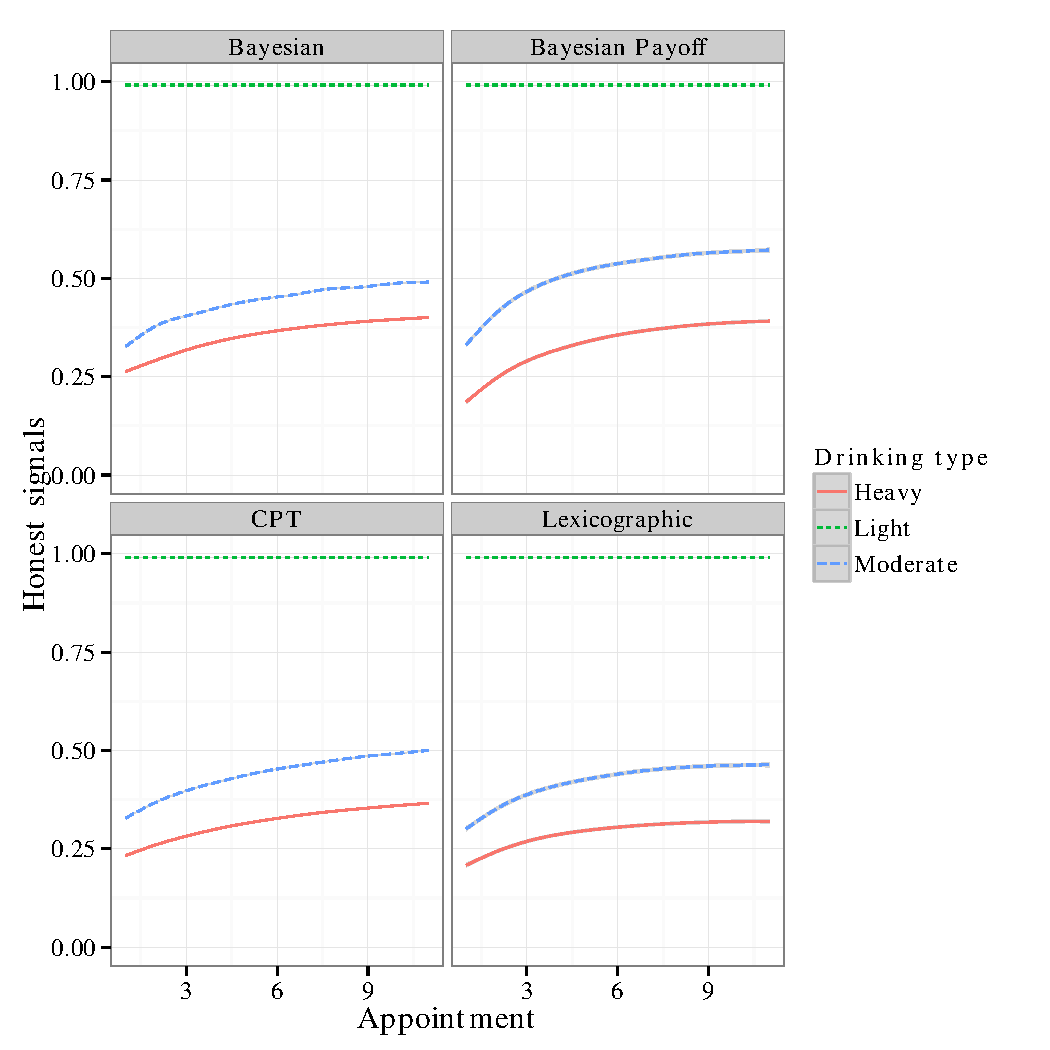
\includegraphics[width=100mm]{figures/honesty_plot}
\caption{Average fraction of population ever signalled honestly by each appointment, after 1000 rounds, mean with 95\% confidence limit over 1000 runs. Note that the large number of runs leads to very tight confidence intervals.\label{fig:honest_signals}}
\end{figure}

\subsection{Social Learning}
\label{sub:sharing_results}

Introducing social learning amongst women leads the behaviour of the decision rules to diverge markedly, which we explore possible reasons for in section \ref{sec:discussion}. Figure \ref{fig:honest_sharing} shows the proportion of women who have signalled honestly at least once by their final appointment, under four sharing conditions. 

\begin{figure}[H]
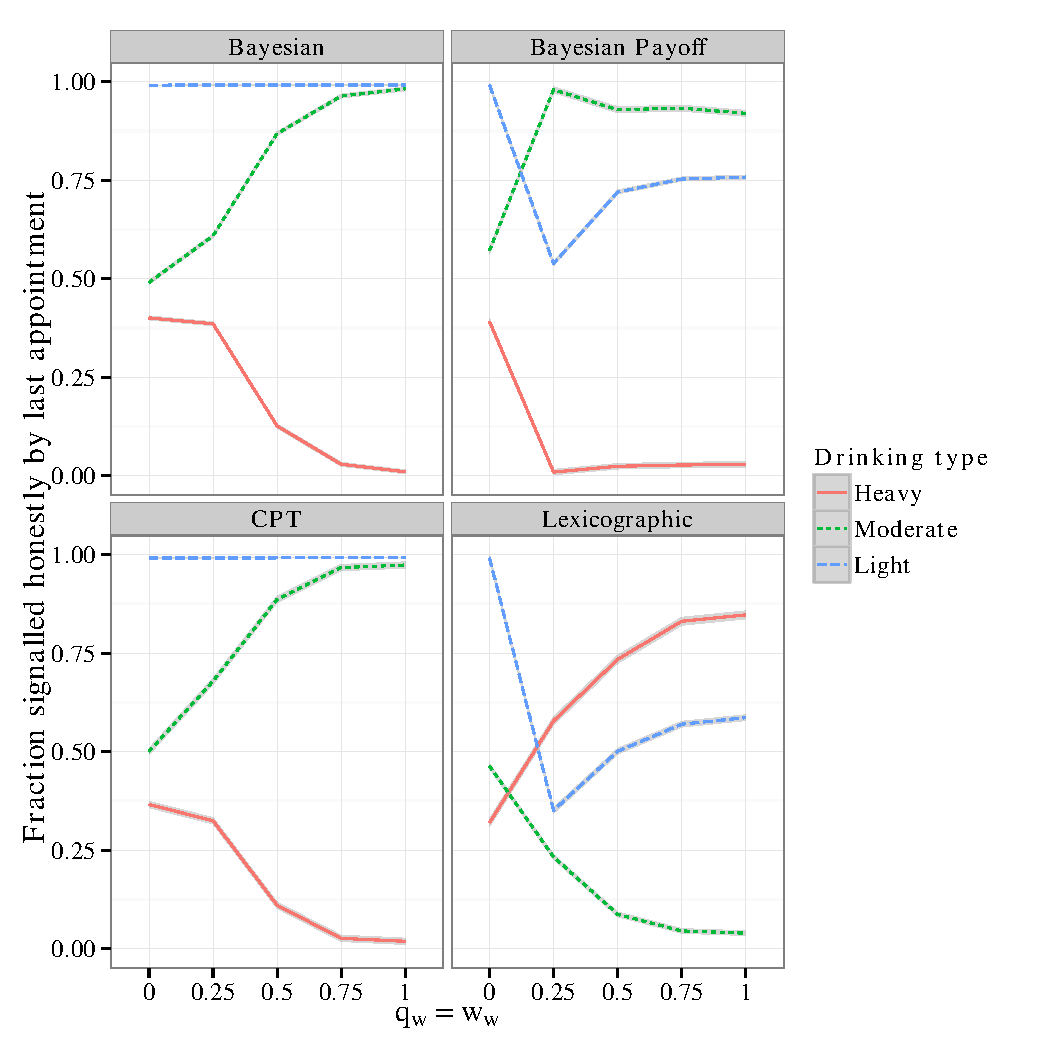
\includegraphics[width=100mm]{figures/honesty_sharing}
\caption{Impact of social learning on trends in the average fraction of population ever signalled honestly by their final appointment, after 1000 rounds, mean with 95\% confidence interval over 100 runs}
\label{fig:honest_sharing}
\end{figure}

Aside from the lexicographic decision rule, the general tendency is towards less honest signalling by heavy drinkers, which is accompanied by a slight increase in referrals for the Bayesian, and \ac{CPT} rules. For these decision models, this is because social learning exacerbates the existing tendency of heavy drinkers to impersonate moderate drinkers, who behave more honestly as heavy drinkers become less so. This arises because both classes of agent learn that the moderate signal is the lower risk option as it is both a reliable indicator of need, and does not attract strongly negative judgement. The reliability of the signal is self reinforcing, since the more the agents use it and get referred, the more confident midwives become that it indicates need.

Particularly notable, is the decline in honest signalling by light drinkers visible in both heuristic type rules at the 0.25 level of \(q_{w}\) \& \(w_{w}\), which is associated with an increase in false positives. This arises because of the lack of homophily in social learning, as light drinkers become informed about negative outcomes associated with concealment, despite having nothing to conceal. The relatively high referral rates of drinkers heighten the effect further, because shared information becomes dominated by their experiences. 

The relationship is not, however, entirely straightforward, in that increasing social learning leads to greater variance between runs. A linear model was used to predict the between-runs interquartile range of the average signal sent by moderate drinkers. The predictors used were decision rule, and level of social learning, together with the interaction between the two. The regression results were significant (\(F_{7,12}=25,p<2.9\times10^{-6}\)) with \(R^2=94\%\), and intercept 0.07. The only significant coefficients were for the interaction terms, which were 0.44 (\(p<0.05\)) for the Bayesian payoff rule, and 0.69 (\(p<0.005\)) for the lexicographic. This suggests that social learning, for the heuristic style decision rules introduces considerable uncertainty to the model, which is explored further in the sensitivity analysis below.


\subsection{Sensitivity Analysis}
\label{sub:sa_results}

In this section we present a brief overview of the sensitivity analysis, followed by selected results highlighting the global effect of changes to perceived payoffs and degree of bias towards honesty, as well as social learning within women. The full results for the sensitivity analysis covering all sixteen emulators are available in appendix \ref{app:sensitivity_results}.

\begin{figure}[H]
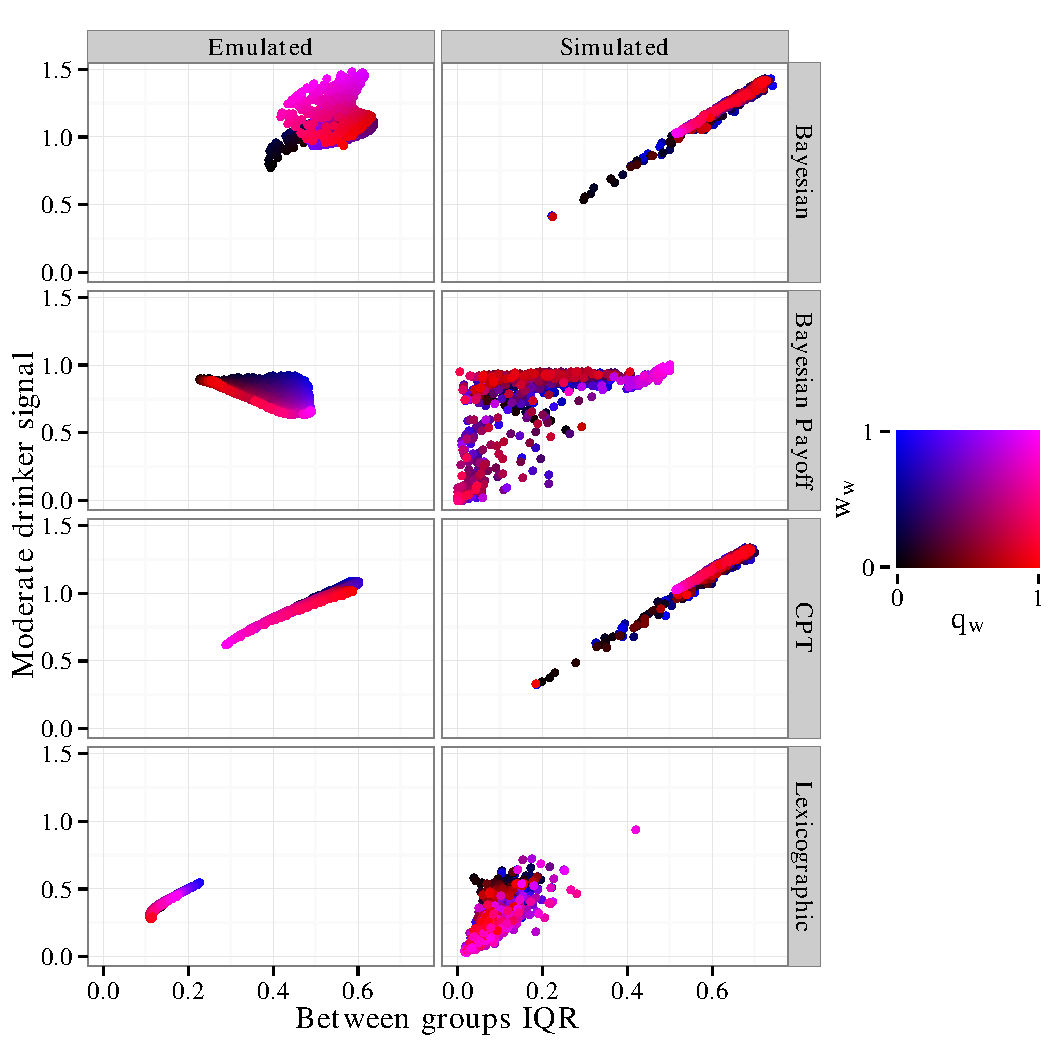
\includegraphics[width=90mm]{figures/sharing_emulated_simulated}
\caption{Median moderate drinker signal vs median between drinking type IQR for all decision rules, with signals coded as 0 = light, 1 = moderate, and 2 = heavy.}
\label{fig:outcome_plots}
\end{figure}

For the median signal choice of moderate drinkers, the results of the sensitivity analysis suggest that the proportion of light drinkers has a significant effect for all decision rules, accounting for 10\%, 38\%, 24\%, and 5\% of the variance in output for the Lexicographic, Bayesian Payoff, Bayesian, and \ac{CPT} rules respectively. For the Lexicographic rule, the overwhelming majority of variance in signalling behaviour is reflective of the prevalence of stigmatisation by midwives (44\% \(p_{m}(m)\), 7\% \(p_{l}(m)\), and a further 15\% for their interaction).  The proportions of midwives are also key drivers in group separation, and the between run IQR of both measures for this rule. 

Perhaps surprisingly, variance attributable to social learning between midwives is relatively low, with neither the weight nor probability accounting for more than 5\% of variance in any measure. While there are small contributions to variance in interaction with other parameters (e.g. 4\% to between groups IQR, for the interaction with the proportion of light drinkers under the Bayesian rule), this may suggest that the model is lacking in this area, which we touch on in section \ref{sec:conclusion}.

Figure \ref{fig:outcome_plots} gives a qualitative picture of both emulator quality, and the divergent response surfaces of the decision rules in response to variations in social learning parameters. Emulator fit is clearly imperfect, but overall behaviour is qualitatively similar, with both emulated and simulated plots demonstrating separation in outcome space for the decision rules.

\begin{figure}[H]
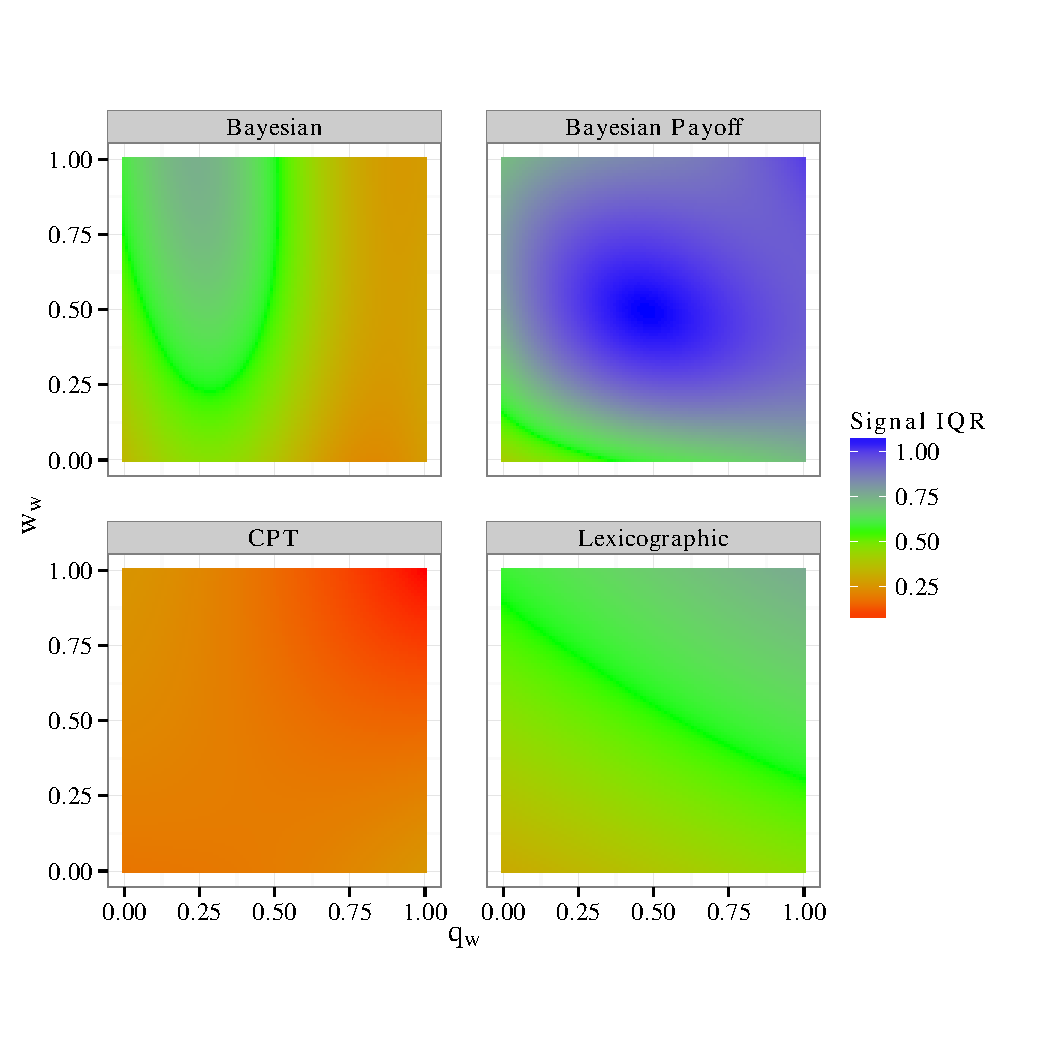
\includegraphics[width=100mm]{figures/unfixed_emu_sig_iqr}
\caption{Emulated moderate drinker signal IQR in response to varying \(q_{w}\), and \(w_{w}\)}
\label{fig:emulated_sharing_iqr}
\end{figure}

Following from the suggestive results for social learning introducing uncertainty (section \ref{sub:sharing_results}), figure \ref{fig:emulated_sharing_iqr} shows emulated points covering the parameter space in high resolution. These plots reflect the increase in uncertainty of outcome shown for the heuristic type rules, which is especially severe for the Bayesian payoff rule. They also suggest that the Bayesian decision rule is less stable under conditions where the weight of shared information is substantially higher than the probability of sharing. This indicates that placing a high weight on information from limited sources leads to greater variability, i.e. what information is shared, matters.

\begin{figure}[H]
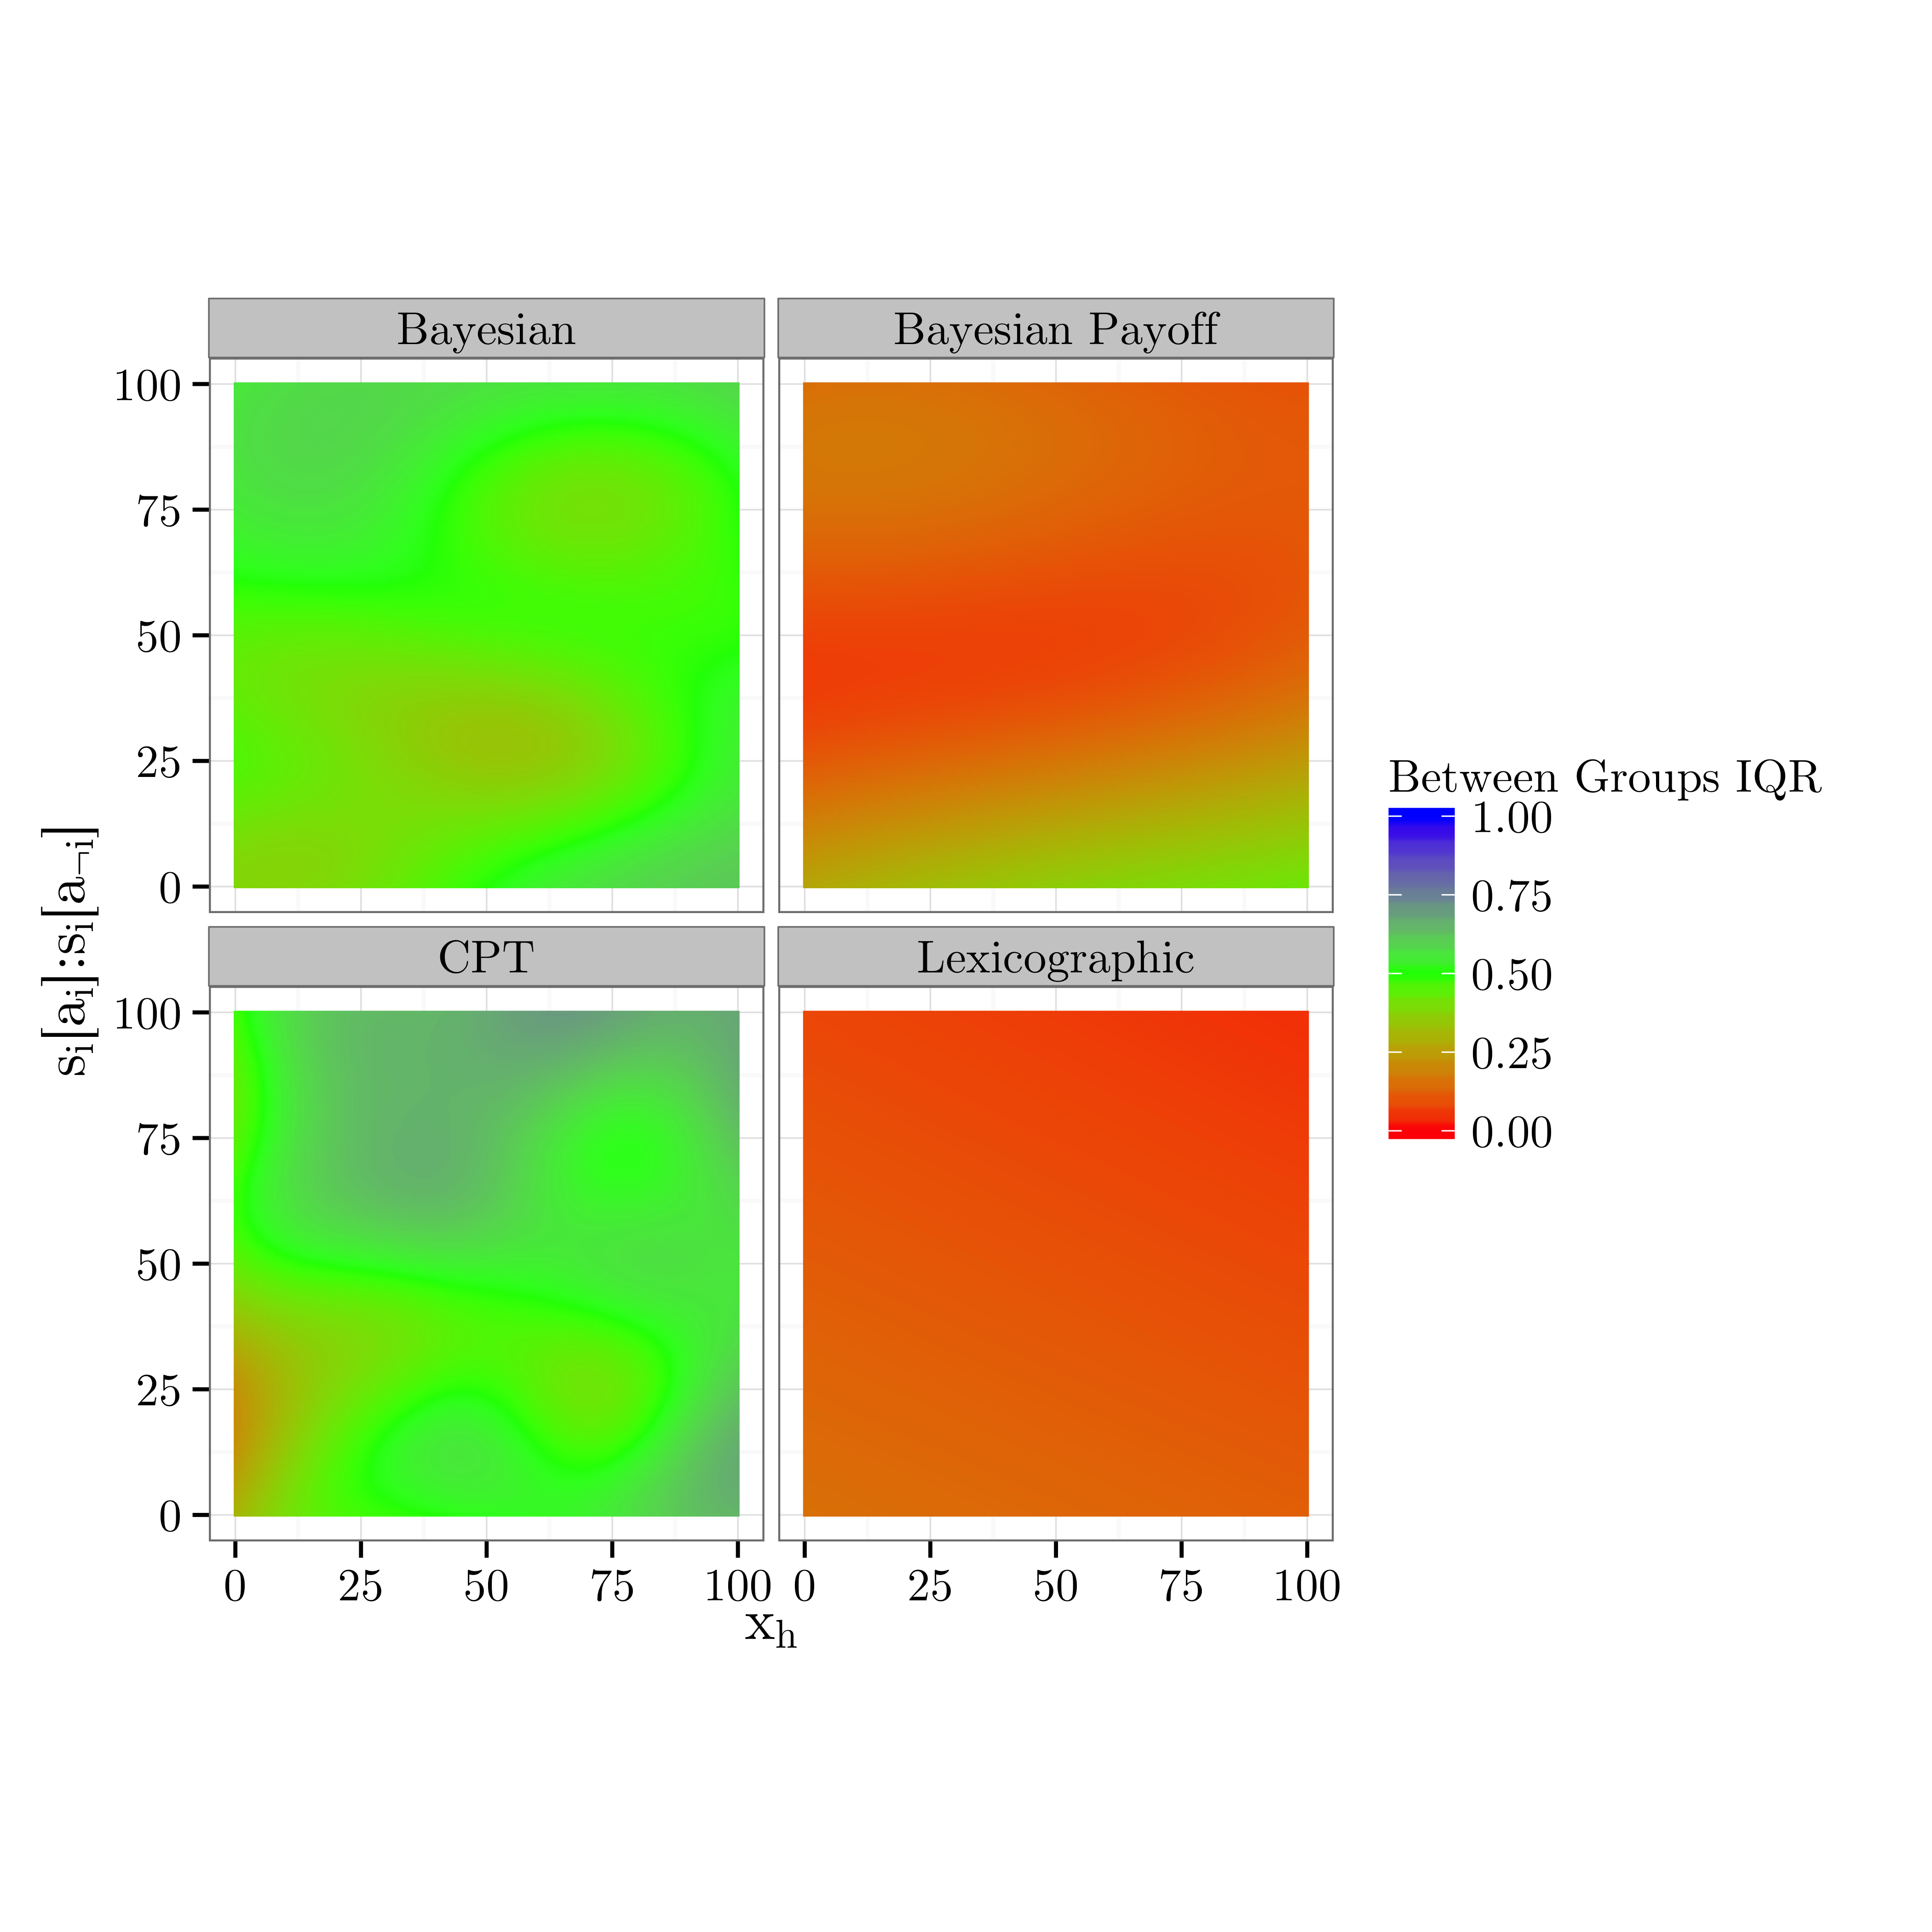
\includegraphics[width=100mm]{figures/unfixed_emu_payoff_honesty_group_iqr}
\caption{Emulated between groups IQR in response to varying \(s_{i}[a_{i}]:s_{i}[a_{\neg i}]\), and \(x_{h}\)}
\label{fig:emulated_payoff_group_iqr}
\end{figure}

For the \ac{CPT}, and Bayesian decision models, the interaction of bias towards honesty, and distinction between payoffs has a significant, and non-linear effect on instability, and separability of groups. Figure \ref{fig:emulated_payoff_group_iqr} shows the effects, and also highlights the tendency towards poor separability of groups for both the heuristic type decision rules. The response surface of the Bayesian payoff rule is slightly more nuanced than the simple Lexicographic rule. Figure \ref{fig:emulated_payoff_group_iqr} shows better separation, close to partial pooling\footnote{Pooling occurs when signallers of different types `pool' their signals, and one adopts the signals of another.} at high payoff distinction, with relatively modest honesty bias, which is reflected by the variance contributions of 11\% and 8\% respectively.  For the more complex rules, the general tendency is towards less pooling for higher values of both, but with pockets where full pooling\footnote{Indicating that all signaller types are using a the same signal.} occurs.  The plots also suggest that the sensitivity of the \ac{CPT} rule is marginally greater, which is supported by the significant contribution to variance of close to 15\% for all measures of \(x_{h}\).
 
\section{Discussion}
\label{sec:discussion}

From a pragmatic perspective, the differing response characteristics of the classes decision rules are substantial and significant, particularly when social learning is considered. There is a high level of uncertainty in the overall dynamics with the model free rules. This does not arise with the more complex rules, because they reframe information from others in the context of their own experiences, as what would happen to them in that situation. By contrast, the simpler rules treat the experiences as having literally happened to them, and since there is no mechanism of homophily, no way to listen only to accounts of agents similar to themselves, they can come to believe unreasonable things. Naturally, incorporating homophily, by, for example weighting shared information by the type of the sharer, would represent a trivial modification to the heuristic models. While to some extent this highlights the flexibility of the decision rule approach, it would of course sacrifice the parsimony of the model. This is an important consideration, given that part of the argument in favour of a decision theoretic approach lies in the minimal nature of the behavioural rules.

One of the notable features of the results is that the behaviour of rules within a class is very similar. To some extent this reflects poorly on the most complex rule, \ac{CPT}, which diverges only minimally in behaviour from the Bayesian model. This might be to a degree anticipated since we have not elicited payoffs for obvious practical and ethical reasons, and they may be unrealistic, which limits the utility of the \ac{CPT} approach.  Additionally, work by \citet{Glockner2012} has shown that there is considerable variation in individual parameters for the decision model, whereas we have let them remain homogeneous here. In the same vein, utility functions should arguably vary between individual agents, which could potentially be addressed by replacing the fixed payoffs used here with a distribution.  With this said, the significant increase in complexity, which entails both additional parameters and increases to simulation time may auger for a middle ground, particularly where elicitation of payoffs is impractical.  This, together with the variability associated with the heuristic type decision rules speaks to a trade off between capturing reality, and replicating it.

Continuing the discussion of the issues raised by the representation of payoffs, the temporal aspect is significant, in that there is a timing difference in payoffs, since while the potential social pain of disclosure is immediate, the health outcome comes only later. In light of this, that there is a known impact of time on perceived utility \citet{Thaler1981} suggests that incorporating some form of temporal discounting (e.g. exponential \citep{Samuelson1937}, or hyperbolic \citep{Ainslie1991}), or a decision model which explicitly treats intertemporal choice, such as the \ac{CPT}-like model of \citet{Loewenstein1992}, is warranted. 

As noted in section \ref{sub:sensitivity}, the impact of social learning in midwives is surprisingly minimal, where it might be expected to play a more significant role in reality. A possible explanation for this lies in the implementation, which may place an excessive constraint on how much information midwives can share. The restriction to sharing only after a referral, together with the disparity in population sizes, and random allocation of appointments leads to midwives rarely having more than a single interaction with woman to pass on to their colleagues. Furthermore, because midwives are only informed of the true type if a referral occurs, they have an inherent myopia since until they have evidence of deception they will not refer, with said evidence difficult to obtain without a referral.

In reality it might be anticipated that midwives would not withhold judgement, and would pass on concerns about specific women to their colleagues, or that particularly dramatic stories would persist and be passed. This might be addressed by incorporating noisy type information \citep{Feltovich2002}, capturing the unintentional information transmitted during appointments, together with a relaxation of the assumptions about when information may be shared and more sophisticated model of information flow in general. This also highlights an advantage of the \ac{BACCO} approach (which we describe in section \ref{sub:sensitivity}), in diagnosing issues with model design by giving insight into parameters which are contributing inappropriately to variance in output. Coupled with the ability of emulators to rapidly explore parameter space, this clearly suggests that statistical emulation is a powerful tool to support simulation based approaches.
As noted in section \ref{sub:sa_results} the emulators here are indicative, but not definitive. Amongst the reasons discrepancy arises here are heteroskedasticity associated with social learning, the stochastic nature of the simulation, and a lack of precision given the large parameter range. The former issues could be addressed by a more comprehensive approach to setting the nugget, which explicitly incorporates point variance.  The latter could be improved through iterative fitting procedures, where the simulation is sampled more heavily in plausible regions of parameter space, a procedure not possible here given the dearth of data to evaluate plausibility. That the discrepancy exists is not prohibitive in this instance, since we are not using the emulator for prediction, only to achieve a broad strokes picture of the behaviour of the simulator.

\section{Conclusion}
\label{sec:conclusion}

The conclusions that can be drawn about the behaviours of real life women, and their midwives, are necessarily limited by the paucity of data available to validate the model. While qualitative trends offer some indication, they are limited in scope, and do not permit strong claims about the drivers of disclosure.  As such, further work will focus on applying the model to domains where validation data is more available, which will support a more comprehensive evaluation of the model discrepancy. 
With this said, the trends reported by \citet{Alvik2006}, and \citet{Phillips2007} are borne out by the model, and predictions from the two more complex rules suggest that encouraging information sharing between women may encourage disclosure, but at the expense of reducing accuracy. By contrast, if one takes the view that a Lexicographic model is a better approximation of real behaviour, then outcomes can best be influenced by controlling how far midwives punish their women socially. We would however suggest that there are better reasons than the outputs of a simulation for doing so.

More broadly, the results demonstrate the logistical feasibility, and its utility as a `tool for thinking', of an agent model grounded in decision theory. The results also make clear that deciding the operationalisation of the decision making is of key significance.

 % Disclosure is a widely applicable issue in health and social care and beyond, with examples ranging from a lack of help seeking behaviour noted in older men \citep{Smith2007a}, to the inverse scenario of innapropriate disclosure in social media \citep{christofides2009information}.
 \section*{Acknowledgements}
\label{sec:acknowledgements}

This work was supported by the Engineering and Physical Sciences Research Council 
(EPSRC) grant EP/H021698/1 Care Life Cycle, funded within the Complexity 
Science in the Real World theme. The authors also gratefully acknowledge the use of the IRIDIS High Performance Computing Facility, and associated support services at the University of Southampton, in the completion of this work. 
\bibliography{library,library_addendum}
\bibliographystyle{spbasic}
\section{Disclosure Game Model Development}
\label{app:model_description}

This appendix provides a more in depth exploration of the model development process, beginning by deriving a game to serve as the basis for the model, and decision problems.

A game, in the game theoretic sense, can be any interaction where the result for one person is dependent on the actions of another. In this scenario, the result for the woman would seem dependent on whether the midwife chooses to refer her for specialist support (although naturally the reality can only be thought of in terms of risk mitigation), and conversely, the right choice for the midwife is somewhat contingent on what the woman is willing to tell them.

A very simple way to represent this would be a game with two players, who both have two possible moves - ask for help, or not; and refer, or not (fig \ref{fig:simplest_game}). Since both parties are invested in the outcome of the pregnancy, we might allow them to share the same payoff if everything ends well.


\begin{figure}[H]
\sidecaption
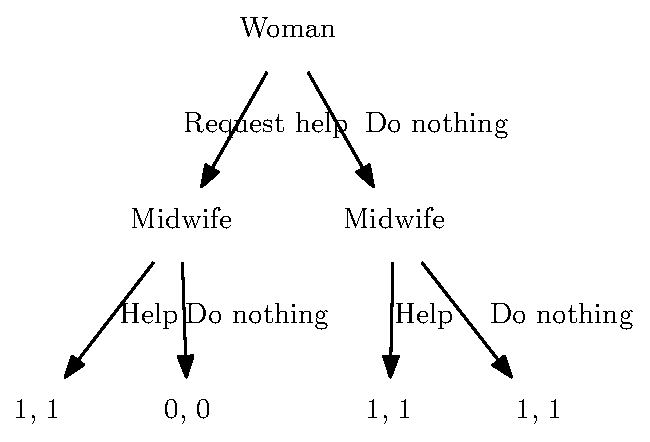
\includegraphics[width=7cm]{figures/simplest_game}
\caption{A very simple two player game. The only time things in this very restricted world obviously end poorly, is if the woman asks for help but does not get any. This implies that a rational player would always refer if asked for help, and is indifferent otherwise - in other words, there are three possible Nash equilibriums\protect\footnotemark.}
\label{fig:simplest_game}
\end{figure}

\footnotetext{A Nash equilibrium is a solution to a game between two or more players, where no player can gain from changing their move.}

The first complication, is that there should be differentiation between referring, and doing nothing because specialist treatment incurs a cost. We can modify the payoffs to reflect this, by reducing the midwife's payoffs when they refer. If the cost of referring is less than the value of a good outcome, then the effect of this is to make the only rational choice when not asked for help is to do nothing.

This simple game is however not very informative, and clearly neglects much of the nuance of the scenario. The wider difficulty here is that the real outcome depends on an attribute of one of the players, rather than their moves. In this case, we would expect the right choices to depend on the alcohol consumption of the woman, rather than entirely on what she has claimed about it.
To reflect this, we would need different variations on the same game to reflect this attribute. 

To resolve this, we can do exactly that, and cast it as a signalling game (fig \ref{fig:less_simple}), with three types of player, corresponding to categories of drinking behaviour (light, moderate, and heavy). Each of these types of player, will play a different game. This also introduces a third player, who we will call nature. Nature takes the first move, and decides the type of the woman according to some probability distribution; in this case we will allow the probability of types to be uniform. 
This changes the dynamics of play substantially, since the midwife can no longer be certain of which game they are playing, and hence which move yields the best outcome. We must also amend the moves, and payoffs slightly. The woman now claims to be one of the types, and may send a signal to say, for example, that she a heavy drinker. We will also modify the common payoffs to allow light drinkers to get the best outcome no matter what, and moderate and heavy types to get the best outcome only if referred. We can also differentiate between the consequences of not getting help for these types by letting heavy drinkers have a very negative outcome, and moderate drinkers a slight one.

\begin{figure}[H]
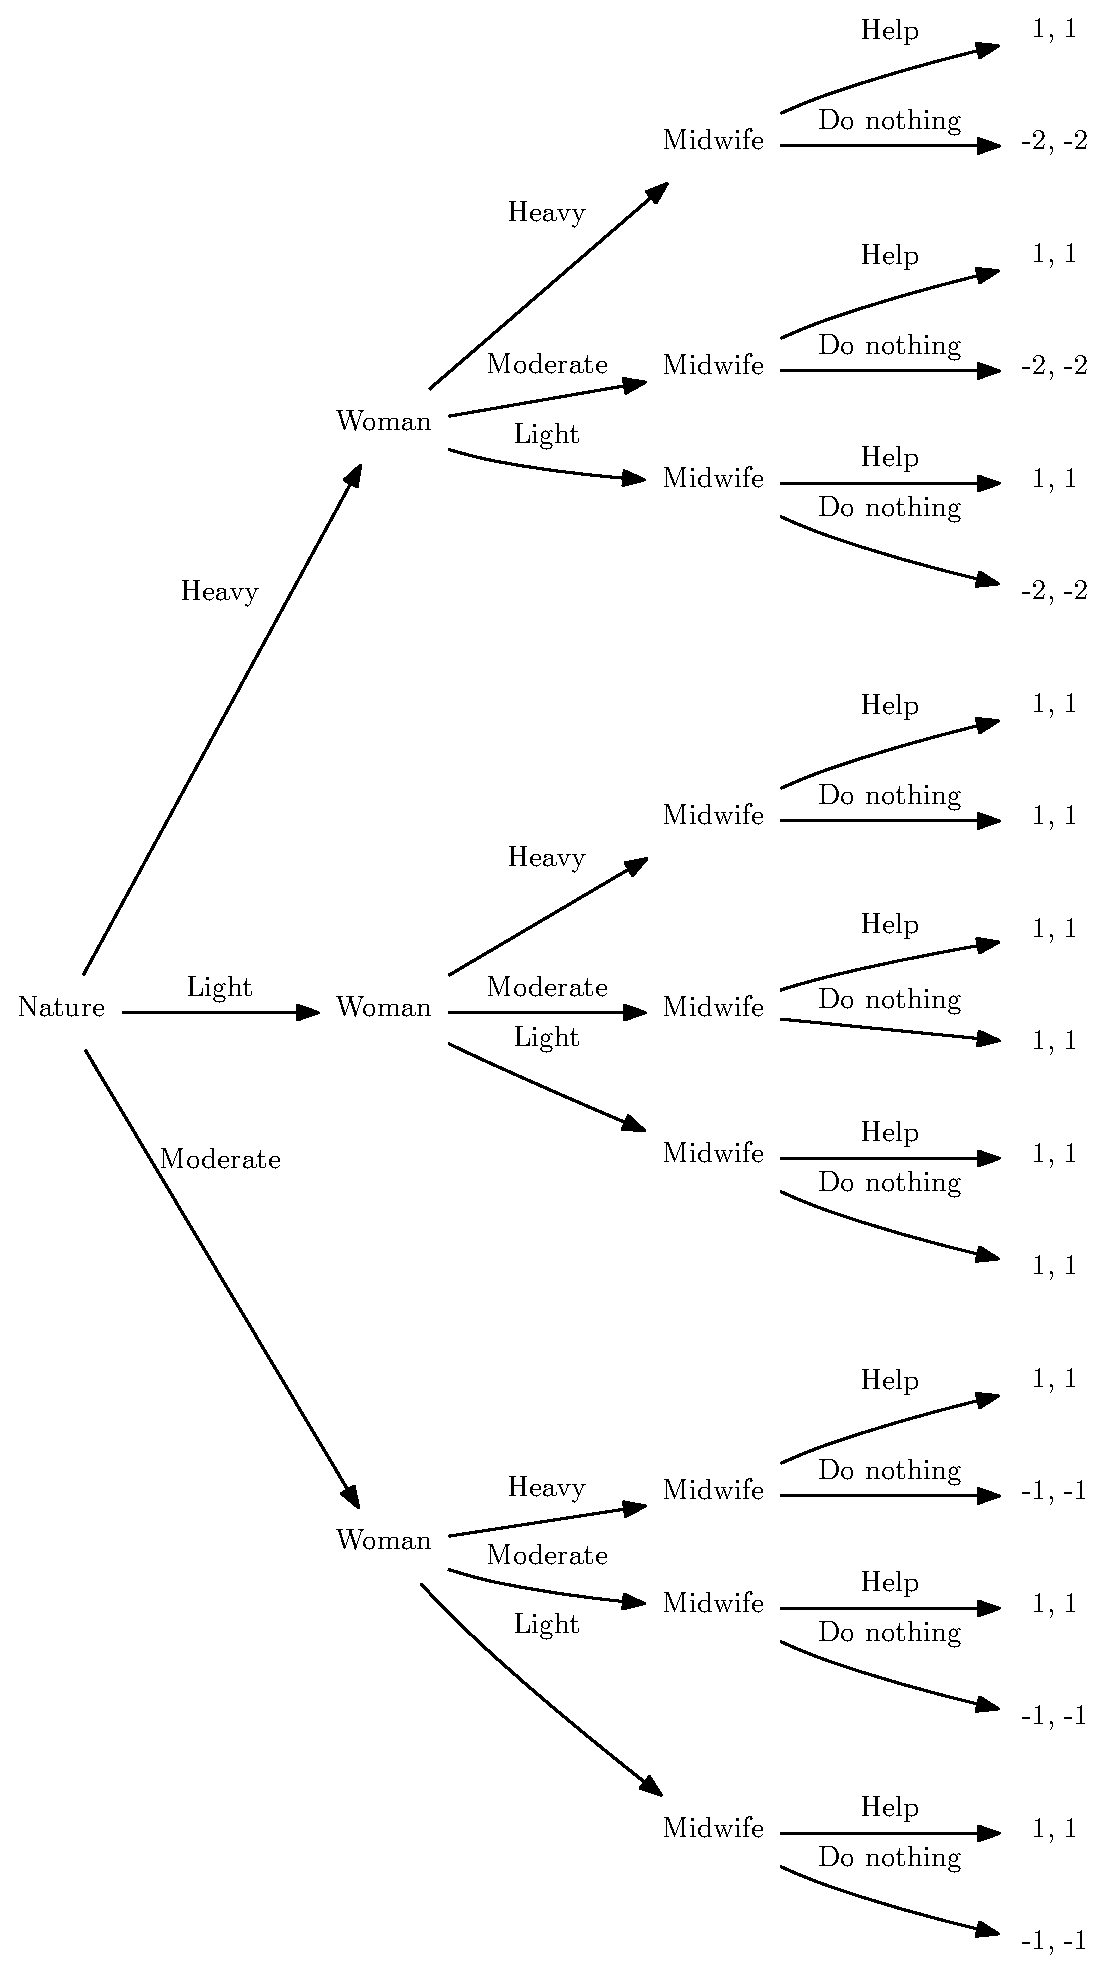
\includegraphics[width=\textwidth]{figures/less_simplest_game}
\caption{A less simple two player signalling game. }

\label{fig:less_simple}
\end{figure}

At this point, the game becomes challenging to analyse from a Nash equilibrium perspective (there are several hundred). But, having raised to issue of stigma, we would also like incorporate this in the game. A possible approach to this is similar to the drinking behaviour of the women, and lets midwives have a type as well, corresponding to how judgemental they are when receiving signals: non-judgemental, moderately judgemental, and harshly judgemental. The expression of this judgement is not a matter of choice on their part, and is assumed to have no impact on their clinical response. Nature now has an additional move, to choose the type of the midwife, and we add costs for sending moderate and heavy signals. A heavy signal to a harshly judgemental midwife adds a heavy cost, and a moderate cost from a moderate midwife. The resulting game might reasonably be said to be intractable.

At this juncture, we do not gain much further from the game representation, and instead separate it into multiple decision problems. 

Breaking the game down into separate decision problems can be achieved by treating the moves of the other players as a chance node, and omitting moves by nature that are known to them. For women, there are two such nodes, corresponding to the move by nature determining the type of midwife they play against, and the midwife's action. Midwives have simpler problem with only a single chance node, because the woman's move is known to them. Figure \ref{fig:decision_problems} shows the structure of the resulting decision problems. Note that there are in fact three distinct decision problems for the three types of woman, since the move by nature determining their type is known to them. 

\begin{figure}[H]
\subfloat[Women (heavy drinkers)]{\includegraphics[width=11.9cm]{figures/women_influence}}
\vskip\baselineskip
\subfloat[Midwives]{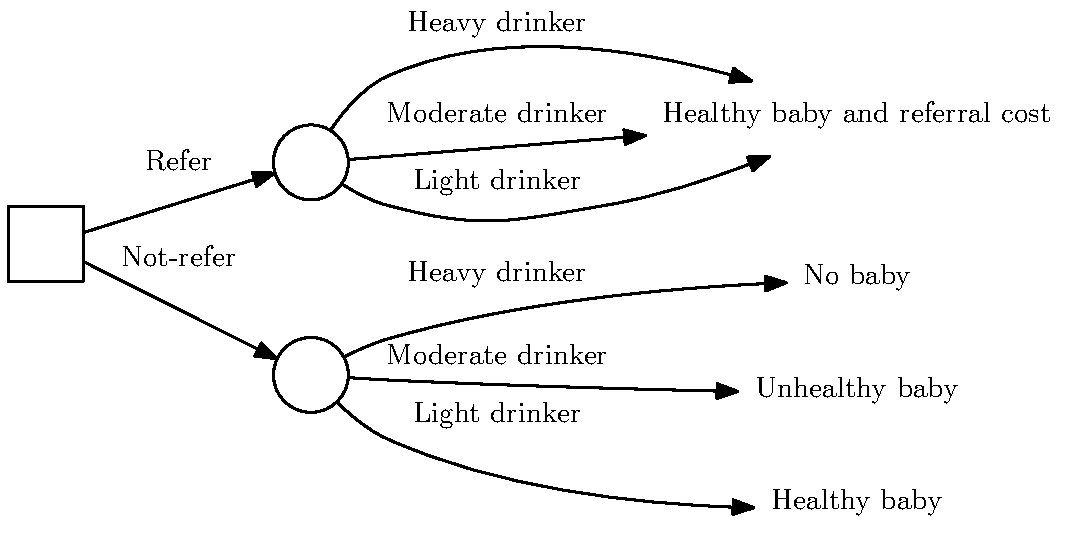
\includegraphics[width=11.9cm]{figures/mw_influence}}
\caption{Influence diagrams, showing the game broken into two decision problems. Squares indicate a decision node, while circles are (from the perspective of the agent) chance nodes}

\label{fig:decision_problems}
\end{figure}


The precise structure of the decision problem is to some extent dependent on the decision rule in use, for example the Lexicographic heuristic rule is concerned only with a direct relationship between action and consequence. However, the literal translation from game to decision problem for women yields two chance nodes. As a result, solving this using the heuristic approach requires that the nodes be combined. By the same token, an arbitrarily complex problem could be resolved by rules without this limitation. This is significant, in that the decision problem is an individual agent's model of the situation, which might not be expected to correspond perfectly with the true sequence of events.

From this position, simulating play, and augmenting the basic conjecture is easily achievable, since together the game, and the decision rules specify the basis for a simulation model. In the disclosure game case, we make additional stipulations on how many games agents play, order of play, the circumstances under which agents observe true types, and the structure of agent populations amongst others.  
\section{Simulation Schedule}
\label{app:sim_schedule}

In this section we give the step by step process for a single run of the disclosure game simulation.

\begin{enumerate}
\item Generate 1000 women, and place them in a queue
\item Generate 100 midwives.
\item For each round of the game
\begin{enumerate}
	\item Take 100 women from the queue
	\item Pair each one with a random midwife
	\item For each pair
	\begin{enumerate}
		\item The woman sends a signal
		\item The midwife refers or not based on the signal
		\item The woman is informed of her payoff, the midwife's type, and whether she is referred
		\item The woman updates her beliefs
		\item The midwife stores the game in their memory
		\item If the woman is referred
		\begin{enumerate}
			\item The midwife is informed of the woman's true type
			\item The midwife retrospectively updates their beliefs using the true type, and memories of any games with this woman
			\item The midwife is now eligible to share their memories of games with this woman
		\end{enumerate}
	\end{enumerate}
	\item Women who have not been referred or had their baby, join the back of the queue
	\item New women are generated to replace those referred, or delivered
	\item The new women are added to the back of the queue
	\item For each referred or birthed woman
	\begin{enumerate}
		\item With probability p, her memory of games is shared with the active women
		\item She is removed from simulation
	\end{enumerate}
	\item The active women update their beliefs
	\item For each midwife with information to share
	\begin{enumerate}
		\item With probability p, their memory of games with the referred woman is shared
		\item The memory is no longer eligible to be shared
	\end{enumerate}
	\item The midwives update their beliefs
\end{enumerate}
\end{enumerate} \section{Agent Examples}
\label{sec:agent_eg}

This section provides a worked example for the learning and decision process of each agent model, focusing on the behaviour of the signalling agent.

\subsection{Lexicographic Heuristic}
\label{sub:lexico_eg}

As an example, take a light drinker who has played three rounds with a succession of particularly judgemental midwives, signalling honestly in two and claiming to be a moderate drinker in one. The most common outcome of the honest signal was a payoff of 10, which is clearly preferable to the 9 gained by claiming to be moderate. On that basis, they choose to signal honestly.

\subsection{Bayesian Payoff}
\label{sub:payoff_eg}

If we take our light drinker from the lexicographic case, and assume that they began with an uninformative prior. The 6 possible signal-payoffs pairings are then \([(l,10),(m,10),(h,10),(m,9),(h,9),(h,8)]\), with \(\alpha_{i}=1\) for all \(i\). After playing the three rounds, \(n_{l,10}=2\), and \(n_{m,9}=1\).

The agent then evaluates \(R_{w}\) for each signal, e.g. for the light signal:

\begin{equation*}
\begin{aligned}
X &= \{10\}\\
R_{w}(l) &= \sum_{x \in X} -xp(x | l) = -10p(10 | l)\\
R_{w}(l) &= -10(\frac{\alpha_{l,10}+n_{l,10}}{\sum_{j}(\alpha_{j}+n_{j})}) = -10(\frac{1+2}{1+2})\\
R_{w}(l) &= -10(\frac{3}{3}) = -10
\end{aligned}
\end{equation*}

and by the same method, \(R_{w}(m)=-9\frac{1}{3}\), and \(R_{w}(h)=-9\), concluding that signalling honestly is the best move.

\subsection{Bayesian Risk Minimisation}
\label{sub:bayes_eg}

Returning to our example agent, under this model the type of the midwife becomes salient, hence \(n_{h}=3\), and \(n_{l,n}=2\), \(n_{m,n}=1\). Their prior beliefs remain uninformative, i.e. \(\alpha_{j} = 1, j \in \{l,m,h\}\), \(\alpha_{i,j}=1,i \in \{r,n\}, j \in \{l,m,h\}\). As before, the agent evaluates \(R_{w}\) for the three signals, and the process for the light signal is given below.

\begin{equation*}
\begin{aligned}
R_{w}(l, l) &= \sum_{i\in A_{m}}\sum_{j\in \Theta} -u_{w}(l, i, l, j)p(j)p(i | l)\\
R_{w}(l, l) &= -u_{w}(l, r, l, l)p(l)p(r | l) - u_{w}(l, n, l, l)p(l)p(n | l)\\
&\phantom{{}=1}- u_{w}(l, r, l, m)p(m)p(r | l)- u_{w}(l, n, l, m)p(m)p(n | l)\\
&\phantom{{}=1}- u_{w}(l, r, l, h)p(h)p(r | l) - u_{w}(l, n, l, h)p(h)p(n | l)\\
u_{w}(l, i, l, j) &= 10\\
R_{w}(l, l) &= -10p(l)p(r | l) - 10p(l)p(n | l) - 10p(m)p(r | l) - 10p(m)p(n | l)\\
&\phantom{{}=1} - 10p(h)p(r | l) - 10p(h)p(n | l)\\
p(l) &= \frac{1 + 0}{1 + 1 + 1 + 3} = \frac{1}{6}\\
p(m) &= \frac{1 + 0}{1 + 1 + 1 + 3} = \frac{1}{6}\\
p(h) &= \frac{1 + 3}{1 + 1 + 1 + 3} = \frac{2}{3}\\
p(r | l) &= \frac{1 + 0}{1 + 1 + 2} = \frac{1}{4}\\
p(n | l) &= \frac{1 + 2}{1 + 1 + 2} = \frac{3}{4}\\
R_{w}(l, l) &= -10\cdot \frac{1}{6} \cdot \frac{1}{4} - 10\cdot \frac{1}{6} \cdot \frac{3}{4} - 10\cdot \frac{1}{6} \cdot \frac{1}{4} - 10\cdot \frac{1}{6} \cdot \frac{3}{4} - 10\cdot \frac{2}{3} \cdot \frac{1}{4} - 10\cdot \frac{2}{3} \cdot \frac{3}{4}\\
&= -10
\end{aligned}
\end{equation*}

and similarly for moderate (\(R_{w}(m,l)=-9\frac{1}{3}\)), and heavy (\(R_{w}(h,l)=-8\frac{1}{2}\)) signals, once again concluding that honesty is the better option.

\subsection{Descriptive Decision Theory}
\label{sub:cpt_eg}

Once again, we return to the light drinker example.  The inferential aspects are identical with the more complex Bayesian risk minimisation algorithm, hence \(p(j)p(i | l)\), and \(u_{w}(l, i, l, j)\) remain the same, but the agent additionally calculates $v(u_{w}(l, i, l, j))w^{+}(p(j))w^{+}(p(i | l))$. For the \ac{CPT} parameters, the values are those originally given by \citet{Tversky1992} and used in the actual simulations which are given in table \ref{tab:cpt_params}.

\begin{table}[H]
\caption{\ac{CPT} parameters. \label{tab:cpt_params}}
\begin{tabular}{llc}
\hline
Name & Description & Value \\ \hline
\(\gamma\) & Probability weighting for gains  & 0.61 \\ \hline
\(\delta\) & Probability weighting for losses &  0.69\\ \hline
\(\alpha\) & Power for gains  & 0.88 \\ \hline
\(\beta\) & Power for losses & 0.88 \\ \hline
\(\lambda\) & Loss aversion &  2.25 \\ \hline
\end{tabular}
\end{table}

\begin{align*}
\alpha &= 0.88\\
\gamma &= 0.61\\
p(l) &= \frac{1}{6}\\
p(m) &= \frac{1}{6}\\
p(h) &= \frac{2}{3}\\
p(r | l) &= \frac{1}{4}\\
p(n | l) &= \frac{3}{4}\\
u_{w}(l, i, l, j) &= 10\\
f&=(10;\frac{1}{24},10;\frac{1}{8},10;\frac{1}{24},10;\frac{1}{8},10;\frac{1}{6},10;\frac{1}{2})\\
f^{+}&=f,f^{-}=()\\
n &= 5\\
v(u_{w}) &= f(u_{w}) = u_{w}^\alpha\\
v(u_{w}) &= 10^{0.88} = 7.59\\
\pi_{0}^{+}&=w^{+}(\frac{1}{24} + \frac{1}{8} + \frac{1}{24} + \frac{1}{8} + \frac{1}{6} + \frac{1}{2}) - w^{+}(\frac{1}{8} + \frac{1}{24} + \frac{1}{8} + \frac{1}{6} + \frac{1}{2})\\
&=w^{+}(1) - w^{+}(\frac{23}{24})\\
&=0.19\\
\pi_{1}^{+}&=w^{+}(\frac{1}{8} + \frac{1}{24} + \frac{1}{8} + \frac{1}{6} + \frac{1}{2}) - w^{+}(\frac{1}{24} + \frac{1}{8} + \frac{1}{6} + \frac{1}{2})\\
&=w^{+}(\frac{23}{24}) - w^{+}(\frac{5}{6})\\
&= 0.17\\
\pi_{2}^{+}&=w^{+}(\frac{1}{24} + \frac{1}{8} + \frac{1}{6} + \frac{1}{2}) - w^{+}(\frac{1}{8} + \frac{1}{6} + \frac{1}{2})=w^{+}(\frac{5}{6}) - w^{+}(\frac{19}{24})\\
&= 0.04\\
\pi_{3}^{+}&=w^{+}(\frac{1}{8} + \frac{1}{6} + \frac{1}{2}) - w^{+}(\frac{1}{6} + \frac{1}{2})=w^{+}(\frac{19}{24}) - w^{+}(\frac{2}{3})\\
&= 0.09\\
\pi_{4}^{+}&=w^{+}(\frac{1}{6} + \frac{1}{2}) - w^{+}(\frac{1}{2})=w^{+}(\frac{2}{3}) - w^{+}(\frac{1}{2})\\
&= 0.09\\
\pi_{5}^{+}&=w^{+}(\frac{1}{2})\\
&= 0.42\\
V(f) &= V(f^{+}) + V(f^{-}) = V(f^{+}) + 0\\
V(f^{+}) &= \sum_{i}^{n}\pi_{i}^{+}(f^{+})v_{i}^{+}(f^{+}) = 7.59
\end{align*}


And as before, following the same process for moderate, and heavy signals which yields respectively 7.14, and 6.22, the agent chooses the higher valued action and sends an honest signal. 
\section{Supplementary Figures}
\label{app:additional_figures}

\begin{figure}[H]
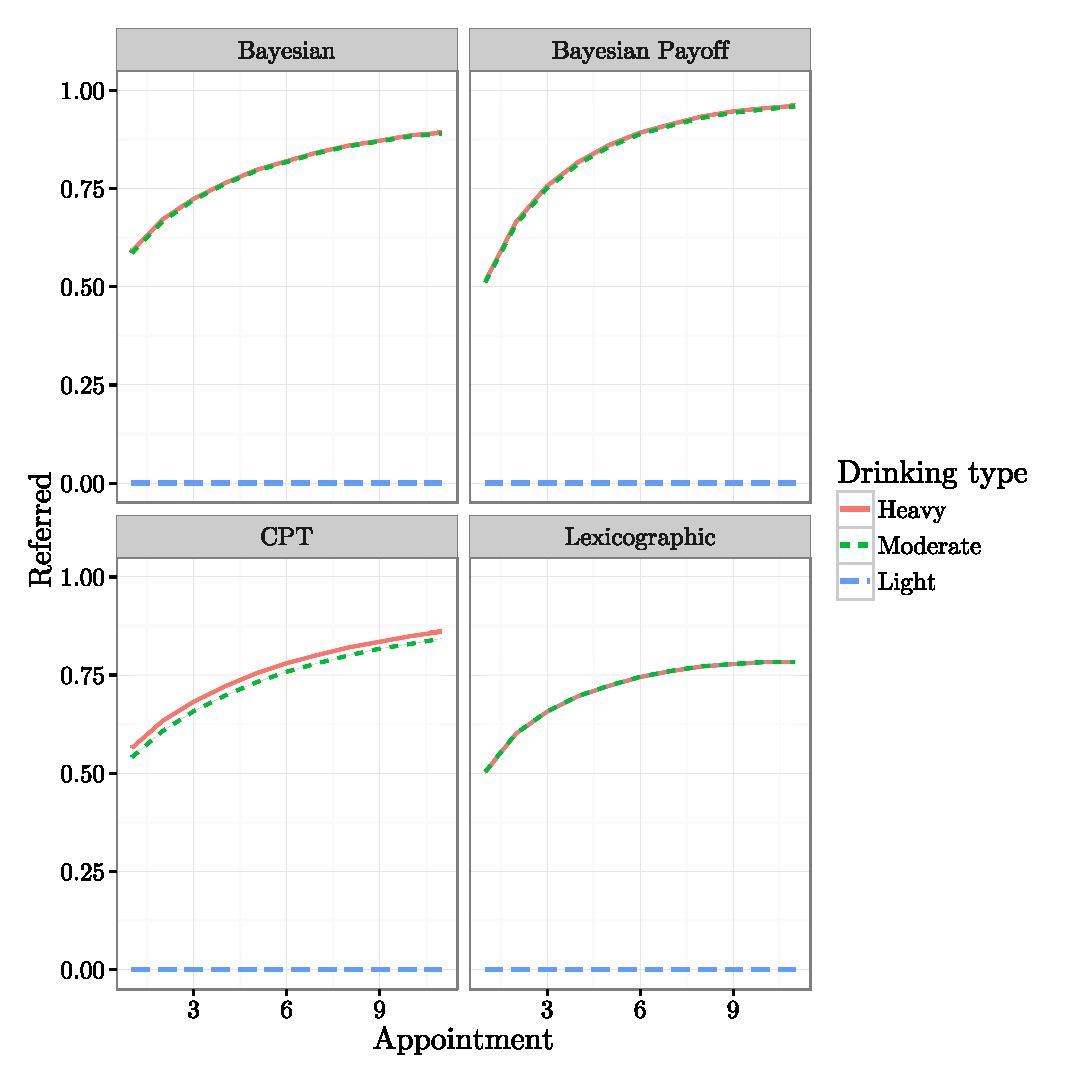
\includegraphics[width=100mm]{figures/ref_plot}
\caption{Average fraction of population referred by each appointment, after 1000 rounds, mean with 95\% confidence limit over 1000 runs. Note that the large number of runs leads to very tight confidence intervals.\label{fig:ref_plot}}
\end{figure} \section{Sensitivity Analysis}
\label{app:sensitivity_results}

This section provides complete variance based sensitivity analysis results for the disclosure game model. Each subsection gives results for one simulation output under all four decision rules, with tables providing the percentage of overall variance attributable to the individual parameters, emulator quality statistics, and the 5 most significant interaction contributions to variance in the output.

\subsection{Median Moderate Drinker Signalling}

\begin{table}[H]
\caption{Median moderate drinker signalling parameter sensitivity \label{tab:sa_results_sig}}
\begin{tabular} {llllll}
\hline\noalign{\smallskip}
Parameter & Description & Lexicographic & Bayesian Payoff & Bayesian & \ac{CPT} \\
\noalign{\smallskip}\svhline\noalign{\smallskip}
\(p_{w}(m)\) & Proportion of moderate drinkers & 0.367 & 1.145 & 0.801 & 0.614 \\
\(p_{w}(l)\) & Proportion of light drinkers & 10.080 & 37.750 & 23.968  & 5.137\\
\(p_{m}(m)\) & Proportion of moderate midwives & 6.715 & 13.017 & 0.894 & 1.485\\
\(p_{m}(l)\) & Proportion of non-judgemental midwives & 43.942 & 1.655 & 1.602 & 2.618 \\
\(q_{w}\) & Probability of women sharing & 0.198 & 5.527 & 4.460 & 1.159 \\
\(w_{w}\) & Weight of shared information for women & 0.355 & 13.025 & 2.716 & 0.888 \\
\(q_{m}\) & Probability of midwives sharing & 0.145 & 0.667 & 0.368 & 0.157 \\
\(w_{m}\) & Weight of shared information for midwives & 0.118 & 0.376 & 0.176 & 0.200 \\
\(x_{h}\) & Health payoff for healthy delivery & 0.457 & 9.618 & 1.912 & 15.355 \\
\(s_{i}[a_{i}]:s_{i}[a_{\neg i}]\) & Pseudo-count favouring honesty & 0.140 & 7.537 & 10.427 & 7.795 \\
Total & All parameters and two way interactions & 86.777 & 96.527 & 85.529 & 74.123 \\
\noalign{\smallskip}\hline\noalign{\smallskip}
\end{tabular}
\end{table}

\begin{table}[H]
\caption{Median moderate drinker signalling emulator statistics \label{tab:sa_emulator_sig}}
\begin{tabular} {lllllll}
\hline\noalign{\smallskip}
Rule & \(\sigma^2\) & Nugget \(\sigma^2\) & Mean output & Total output variance & Code uncertainty & RMSSE \\
\noalign{\smallskip}\svhline\noalign{\smallskip}
Lexicographic & 0.834 & 0.131 &  0.817 & 0.012 & 0.252 & 1.746 \\
Bayesian Payoff & 1.667 & 0.475 &  0.662 & 0.003 & 0.181 & 3.12 \\
Bayesian & 3.352 & 0.534 & 1.160 & 0.001 & 0.068 & 2.423 \\
\ac{CPT} & 1.503 & 0.331 & 1.241 & 0.002 & 0.101 & 1.842 \\
\noalign{\smallskip}\hline\noalign{\smallskip}
\end{tabular}
\end{table}

\begin{table}[H]
\caption{Top 5 Interaction terms for \ac{CPT} decision rule. \label{tab:sa_interaction_prospect_sig}}
\begin{tabular} {ll}
\hline\noalign{\smallskip}
Parameter & Variance \\ 
\noalign{\smallskip}\svhline\noalign{\smallskip}

\(x_{h}\)*\(s_{i}[a_{i}]:s_{i}[a_{\neg i}]\) & 20.814\\
\(p_{w}(l)\)*\(s_{i}[a_{i}]:s_{i}[a_{\neg i}]\) & 5.698\\
\(p_{w}(l)\)*\(x_{h}\) & 2.895\\
\(s_{i}[a_{i}]:s_{i}[a_{\neg i}]\)*\(w_{w}\) & 2.799\\
\(s_{i}[a_{i}]:s_{i}[a_{\neg i}]\)*\(q_{m}\) & 1.686\\
\noalign{\smallskip}\hline\noalign{\smallskip}
\end{tabular}
\end{table}

\begin{table}[H]
\caption{Top 5 Interaction terms for Bayesian decision rule. \label{tab:sa_interaction_sharing_sig}}
\begin{tabular} {ll}
\hline\noalign{\smallskip}
Parameter & Variance \\
\noalign{\smallskip}\svhline\noalign{\smallskip}
\(p_{w}(l)\)*\(s_{i}[a_{i}]:s_{i}[a_{\neg i}]\) & 17.270\\
\(p_{w}(l)\)*\(q_{m}\) & 6.054\\
\(q_{m}\)*\(w_{w}\) & 3.814\\
\(s_{i}[a_{i}]:s_{i}[a_{\neg i}]\)*\(q_{m}\) & 3.538\\
\(s_{i}[a_{i}]:s_{i}[a_{\neg i}]\)*\(w_{w}\) & 3.084\\
\noalign{\smallskip}\hline\noalign{\smallskip}
\end{tabular}
\end{table}

\begin{table}[H]
\caption{Top 5 Interaction terms for Lexicographic decision rule. \label{tab:sa_interaction_lexic_sig}}
\begin{tabular} {ll}
\hline\noalign{\smallskip}
Parameter & Variance \\
\noalign{\smallskip}\svhline\noalign{\smallskip}
\(p_{m}(l)\)*\(p_{m}(m)\) & 15.331\\
\(p_{m}(m)\)*\(p_{w}(l)\) & 3.682\\
\(p_{m}(l)\)*\(p_{w}(l)\) & 3.581\\
\(p_{m}(m)\)*\(q_{m}\) & 0.349\\
\(p_{m}(l)\)*\(q_{m}\) & 0.279\\
\noalign{\smallskip}\hline\noalign{\smallskip}
\end{tabular}
\end{table}

\begin{table}[H]
\caption{Top 5 Interaction terms for Bayesian Payoff decision rule. \label{tab:sa_interaction_payoff_sig}}
\begin{tabular} {ll}
\hline\noalign{\smallskip}
Parameter & Variance \\
\noalign{\smallskip}\svhline\noalign{\smallskip}
\(p_{w}(l)\)*\(w_{w}\) & 4.045\\
\(x_{h}\)*\(s_{i}[a_{i}]:s_{i}[a_{\neg i}]\) & 1.856\\
\(p_{w}(l)\)*\(q_{m}\) & 1.231\\
\(s_{i}[a_{i}]:s_{i}[a_{\neg i}]\)*\(q_{m}\) & 0.997\\
\(q_{m}\)*\(w_{w}\) & 0.929\\ 
\noalign{\smallskip}\hline\noalign{\smallskip}
\end{tabular}
\end{table}

 
\subsection{Median Between Groups IQR}

\begin{table}[H]
\caption{Median between groups IQR parameter sensitivity \label{tab:sa_results_iqr}}
\begin{tabular} {llllll}
\hline\noalign{\smallskip}
Parameter & Description & Lexicographic & Bayesian Payoff & Bayesian & \ac{CPT} \\
\noalign{\smallskip}\svhline\noalign{\smallskip}
\(p_{w}(m)\) & Proportion of moderate drinkers & 0.327 & 0.688 & 0.457 & 0.586 \\
\(p_{w}(l)\) & Proportion of light drinkers & 11.223 & 20.123 & 11.046 & 4.081 \\
\(p_{m}(m)\) & Proportion of moderate midwives & 36.630 & 1.160 & 0.364 & 1.945 \\
\(p_{m}(l)\) & Proportion of non-judgemental midwives & 6.228 & 4.487 & 0.0964 & 2.627\\
\(q_{w}\) & Probability of women sharing & 0.498 & 0.235 & 2.537 & 1.812 \\
\(w_{w}\) & Weight of shared information for women & 1.018 & 2.307 & 1.889 & 0.740 \\
\(q_{m}\) & Probability of midwives sharing & 0.158 & 0.343 & 0.387 & 0.156 \\
\(w_{m}\) & Weight of shared information for midwives & 0.076 & 0.973 & 0.125 & 0.213 \\
\(x_{h}\) & Health payoff for healthy delivery & 0.317 & 10.960 & 3.305 & 16.493 \\
\(s_{i}[a_{i}]:s_{i}[a_{\neg i}]\) & Pseudo-count favouring honesty & 1.107 & 8.411 & 2.890 & 6.729 \\
Total & All parameters and two way interactions & 81.702 & 83.693 & 47.449 & 71.032 \\
\noalign{\smallskip}\hline\noalign{\smallskip}
\end{tabular}
\end{table}

\begin{table}[H]
\caption{Median between groups IQR emulator statistics \label{tab:sa_emulator_iqr}}
\begin{tabular} {lllllll}
\hline\noalign{\smallskip}
Rule & \(\sigma^2\) & Nugget \(\sigma^2\) & Mean output & Total output variance & Code uncertainty & RMSSE \\
\noalign{\smallskip}\svhline\noalign{\smallskip}
Lexicographic & 0.930 & 0.240 & 0.249 & 0.002 & 0.040 & 1.832 \\
Bayesian Payoff & 1.242 & 0.417 & 0.232 & 0.001 & 0.0034 & 2.308 \\
Bayesian & 1.254 & 0.131 & 0.644 & 0.000 & 0.019 & 1.167 \\
\ac{CPT} & 1.190 & 0.313 & 0.659 & 0.000 & 0.024 & 1.701 \\
\noalign{\smallskip}\hline\noalign{\smallskip}
\end{tabular}
\end{table}

\begin{table}[h]
\caption{Top 5 Interaction terms for \ac{CPT} decision rule.}
\label{tab:sa_interaction_prospect_group_iqr}
\begin{tabular} {ll}
\hline\noalign{\smallskip}
Parameter & Variance \\ 
\noalign{\smallskip}\svhline\noalign{\smallskip}

\(x_{h}\)*\(s_{i}[a_{i}]:s_{i}[a_{\neg i}]\) & 19.551\\
\(p_{w}(l)\)*\(s_{i}[a_{i}]:s_{i}[a_{\neg i}]\) & 3.838\\
\(s_{i}[a_{i}]:s_{i}[a_{\neg i}]\)*\(w_{w}\) & 2.450\\
\(p_{w}(l)\)*\(x_{h}\) & 2.337\\
\(s_{i}[a_{i}]:s_{i}[a_{\neg i}]\)*\(q_{m}\) & 2.046\\
\noalign{\smallskip}\hline\noalign{\smallskip}
\end{tabular}
\end{table}

\begin{table}[H]
\caption{Top 5 Interaction terms for Bayesian decision rule. \label{tab:sa_interaction_sharing_group_iqr}}
\begin{tabular} {ll}
\hline\noalign{\smallskip}
Parameter & Variance \\
\noalign{\smallskip}\svhline\noalign{\smallskip}
\(s_{i}[a_{i}]:s_{i}[a_{\neg i}]\)*\(q_{m}\) & 4.284\\
\(p_{w}(l)\)*\(q_{m}\) & 3.866\\
\(p_{w}(l)\)*\(s_{i}[a_{i}]:s_{i}[a_{\neg i}]\) & 2.943\\
\(x_{h}\)*\(s_{i}[a_{i}]:s_{i}[a_{\neg i}]\) & 2.680\\
\(q_{m}\)*\(w_{w}\) & 2.282\\
\noalign{\smallskip}\hline\noalign{\smallskip}
\end{tabular}
\end{table}

\begin{table}[H]
\caption{Top 5 Interaction terms for Lexicographic decision rule. \label{tab:sa_interaction_lexic_group_iqr}}
\begin{tabular} {ll}
\hline\noalign{\smallskip}
Parameter & Variance \\
\noalign{\smallskip}\svhline\noalign{\smallskip}
\(p_{m}(l)\)*\(p_{m}(m)\) & 12.046\\
\(p_{m}(m)\)*\(p_{w}(l)\) & 5.054\\
\(p_{m}(l)\)*\(p_{w}(l)\) & 3.005\\
\(p_{m}(l)\)*\(w_{w}\) & 0.819\\
\(p_{m}(m)\)*\(w_{w}\) & 0.757\\
\noalign{\smallskip}\hline\noalign{\smallskip}
\end{tabular}
\end{table}

\begin{table}[H]
\caption{Top 5 Interaction terms for Bayesian Payoff decision rule. \label{tab:sa_interaction_payoff_group_iqr}}
\begin{tabular} {ll}
\hline\noalign{\smallskip}
Parameter & Variance \\
\noalign{\smallskip}\svhline\noalign{\smallskip}
\(p_{w}(l)\)*\(s_{i}[a_{i}]:s_{i}[a_{\neg i}]\) & 12.883\\
\(p_{w}(l)\)*\(w_{w}\) & 5.667\\
\(p_{w}(l)\)*\(x_{h}\) & 2.447\\
\(x_{h}\)*\(s_{i}[a_{i}]:s_{i}[a_{\neg i}]\) & 2.360\\
\(p_{m}(m)\)*\(p_{w}(l)\) & 1.919\\ 
\noalign{\smallskip}\hline\noalign{\smallskip}
\end{tabular}
\end{table}

 
\subsection{Median Moderate Drinker Signalling IQR}

\begin{table}[H]
\caption{IQR of median moderate drinker signalling parameter sensitivity \label{tab:sa_results_sig_iqr}}
\begin{tabular} {llllll}
\hline\noalign{\smallskip}
Parameter & Description & Lexicographic & Bayesian Payoff & Bayesian & \ac{CPT} \\
\noalign{\smallskip}\svhline\noalign{\smallskip}
\(p_{w}(m)\) & Proportion of moderate drinkers & 0.428 & 9.828 & 3.816 & 2.068 \\
\(p_{w}(l)\) & Proportion of light drinkers & 8.369 & 13.791 & 4.045 & 2.400 \\
\(p_{m}(m)\) & Proportion of moderate midwives & 13.416 & 0.712 & 0.676 & 0.583 \\
\(p_{m}(l)\) & Proportion of non-judgemental midwives & 21.079 & 0.648 & 0.659 & 0.373 \\
\(q_{w}\) & Probability of women sharing & 2.307 & 3.481 & 0.891 & 0.600 \\
\(w_{w}\) & Weight of shared information for women & 6.021 & 6.009 & 0.562 & 0.937 \\
\(q_{m}\) & Probability of midwives sharing & 0.315 & 1.829 & 0.114 & 0.117 \\
\(w_{m}\) & Weight of shared information for midwives & 1.652 & 1.354 & 0.260 & 0.0.139 \\
\(x_{h}\) & Health payoff for healthy delivery & 0.253 & 0.612 & 4.889 & 15.146 \\
\(s_{i}[a_{i}]:s_{i}[a_{\neg i}]\) & Pseudo-count favouring honesty & 0.504 & 3.096 & 19.863 & 25.999 \\
Total & All parameters and two way interactions & 84.9968 & 77.413 & 57.125 & 83.322 \\
\noalign{\smallskip}\hline\noalign{\smallskip}
\end{tabular}
\end{table}

\begin{table}[H]
\caption{IQR of median between groups IQR emulator statistics \label{tab:sa_emulator_sig_iqr}}
\begin{tabular} {lllllll}
\hline\noalign{\smallskip}
Rule & \(\sigma^2\) & Nugget \(\sigma^2\) & Mean output & Total output variance & Code uncertainty & RMSSE \\
\noalign{\smallskip}\svhline\noalign{\smallskip}
Lexicographic & 1.425 & 0.436 & 0.549 & 0.008 & 0.114 & 2.719 \\
Bayesian Payoff & 1.223 & 0.496 & 0.747 & 0.012 & 0.207 & 2.034 \\
Bayesian &  1.065 & 0.000 & 0.230 & 0.002 & 0.088 & 1.015 \\
\ac{CPT} & 0.874 & 0.213 & 0.233 & 0.001 & 0.066 & 1.806 \\
\noalign{\smallskip}\hline\noalign{\smallskip}
\end{tabular}
\end{table}

\begin{table}[H]
\caption{Top 5 Interaction terms for \ac{CPT} decision rule. \label{tab:sa_interaction_prospect_sig_iqr}}
\begin{tabular} {ll}
\hline\noalign{\smallskip}
Parameter & Variance \\ 
\noalign{\smallskip}\svhline\noalign{\smallskip}

\(x_{h}\)*\(s_{i}[a_{i}]:s_{i}[a_{\neg i}]\) & 17.377\\
\(p_{w}(m)\)*\(s_{i}[a_{i}]:s_{i}[a_{\neg i}]\) & 3.356\\
\(s_{i}[a_{i}]:s_{i}[a_{\neg i}]\)*\(w_{w}\) & 3.036\\
\(s_{i}[a_{i}]:s_{i}[a_{\neg i}]\)*\(q_{m}\) & 2.067\\
\(p_{w}(l)\)*\(s_{i}[a_{i}]:s_{i}[a_{\neg i}]\) & 1.721\\
\noalign{\smallskip}\hline\noalign{\smallskip}
\end{tabular}
\end{table}

\begin{table}[H]
\caption{Top 5 Interaction terms for Bayesian decision rule. \label{tab:sa_interaction_sharing_sig_iqr}}
\begin{tabular} {ll}
\hline\noalign{\smallskip}
Parameter & Variance \\
\noalign{\smallskip}\svhline\noalign{\smallskip}
\(p_{w}(m)\)*\(s_{i}[a_{i}]:s_{i}[a_{\neg i}]\) & 4.188\\
\(x_{h}\)*\(s_{i}[a_{i}]:s_{i}[a_{\neg i}]\) & 3.120\\
\(s_{i}[a_{i}]:s_{i}[a_{\neg i}]\)*\(q_{m}\) & 2.423\\
\(p_{w}(l)\)*\(s_{i}[a_{i}]:s_{i}[a_{\neg i}]\) & 2.279\\
\(p_{w}(l)\)*\(q_{m}\) & 1.489\\
\noalign{\smallskip}\hline\noalign{\smallskip}
\end{tabular}
\end{table}

\begin{table}[H]
\caption{Top 5 Interaction terms for Lexicographic decision rule. \label{tab:sa_interaction_lexic_sig_iqr}}
\begin{tabular} {ll}
\hline\noalign{\smallskip}
Parameter & Variance \\
\noalign{\smallskip}\svhline\noalign{\smallskip}
\(p_{m}(m)\)*\(p_{w}(l)\) & 12.068\\
\(p_{m}(l)\)*\(p_{w}(l)\) & 6.794\\
\(p_{m}(l)\)*\(p_{m}(m)\) & 5.567\\
\(p_{m}(m)\)*\(q_{m}\) & 0.886\\
\(p_{m}(l)\)*\(q_{m}\) & 0.692\\
\noalign{\smallskip}\hline\noalign{\smallskip}
\end{tabular}
\end{table}

\begin{table}[H]
\caption{Top 5 Interaction terms for Bayesian Payoff decision rule. \label{tab:sa_interaction_payoff_sig_iqr}}
\begin{tabular} {ll}
\hline\noalign{\smallskip}
Parameter & Variance \\
\noalign{\smallskip}\svhline\noalign{\smallskip}
\(p_{w}(l)\)*\(p_{w}(m)\) & 8.357\\
\(p_{w}(l)\)*\(w_{w}\) & 7.431\\
\(p_{w}(l)\)*\(s_{i}[a_{i}]:s_{i}[a_{\neg i}]\) & 4.882\\
\(p_{w}(l)\)*\(q_{m}\) & 2.346\\
\(p_{w}(l)\)*\(w_{m}\) & 2.025\\ 
\noalign{\smallskip}\hline\noalign{\smallskip}
\end{tabular}
\end{table}

 
\subsection{Between Groups IQR IQR}

\begin{table}[H]
\caption{IQR of median between groups IQR parameter sensitivity \label{tab:sa_results_iqr_iqr}}
\begin{tabular} {llllll}
\hline\noalign{\smallskip}
Parameter & Description & Lexicographic & Bayesian Payoff & Bayesian & \ac{CPT} \\
\noalign{\smallskip}\svhline\noalign{\smallskip}
\(p_{w}(m)\) & Proportion of moderate drinkers & 0.691 & 5.926 & 1.053 & 1.265 \\
\(p_{w}(l)\) & Proportion of light drinkers & 3.664 & 17.047 & 4.877 & 3.656 \\
\(p_{m}(m)\) & Proportion of moderate midwives & 41.369 & 1.124 & 0.814 & 0.591 \\
\(p_{m}(l)\) & Proportion of non-judgemental midwives & 7.109 & 0.739 & 0.496 & 0.378 \\
\(q_{w}\) & Probability of women sharing & 1.963 & 2.038 & 0.733 & 0.589 \\
\(w_{w}\) & Weight of shared information for women & 7.932 & 11.193 & 2.289 & 1.960 \\
\(q_{m}\) & Probability of midwives sharing & 0.413 & 1.972 & 0.267 & 0.069\\
\(w_{m}\) & Weight of shared information for midwives & 0.120 & 2.902 & 0.150 & 0.123 \\
\(x_{h}\) & Health payoff for healthy delivery & 0.228 & 3.190 & 6.308 & 14.777 \\
\(s_{i}[a_{i}]:s_{i}[a_{\neg i}]\) & Pseudo-count favouring honesty & 0.673 & 10.411 & 22.901 & 26.340 \\
Total & All parameters and two way interactions & 85.740 & 88.611 & 68.640 & 84.210 \\
\noalign{\smallskip}\hline\noalign{\smallskip}
\end{tabular}
\end{table}

\begin{table}[H]
\caption{IQR of median between groups IQR emulator statistics \label{tab:sa_emulator_iqr_iqr}}
\begin{tabular} {lllllll}
\hline\noalign{\smallskip}
Rule & \(\sigma^2\) & Nugget \(\sigma^2\) & Mean output & Total output variance & Code uncertainty & RMSSE \\
\noalign{\smallskip}\svhline\noalign{\smallskip}
Lexicographic & 0.826 & 0.409 & 0.259 & 0.002 & 0.034 & 2.364 \\
Bayesian Payoff & 3.202 & 0.520 & 0.328 & 0.002 & 0.032 & 2.452 \\
Bayesian & 1.177 & 0.041 & 0.133 & 0.000 & 0.018 & 1.152 \\
\ac{CPT} & 0.874 & 0.118 & 0.126 & 0.000 & 0.017 & 1.570 \\
\noalign{\smallskip}\hline\noalign{\smallskip}
\end{tabular}
\end{table}

\begin{table}[H]
\caption{Top 5 Interaction terms for \ac{CPT} decision rule. \label{tab:sa_interaction_prospect_group_iqr_iqr}}
\begin{tabular} {ll}
\hline\noalign{\smallskip}
Parameter & Variance \\ 
\noalign{\smallskip}\svhline\noalign{\smallskip}

\(x_{h}\)*\(s_{i}[a_{i}]:s_{i}[a_{\neg i}]\) & 18.626\\
\(p_{w}(l)\)*\(s_{i}[a_{i}]:s_{i}[a_{\neg i}]\) & 3.312\\
\(s_{i}[a_{i}]:s_{i}[a_{\neg i}]\)*\(w_{w}\) & 2.823\\
\(s_{i}[a_{i}]:s_{i}[a_{\neg i}]\)*\(q_{m}\) & 2.694\\
\(x_{h}\)*\(q_{m}\) & 1.022\\
\noalign{\smallskip}\hline\noalign{\smallskip}
\end{tabular}
\end{table}

\begin{table}[H]
\caption{Top 5 Interaction terms for Bayesian decision rule. \label{tab:sa_interaction_sharing_group_iqr_iqr}}
\begin{tabular} {ll}
\hline\noalign{\smallskip}
Parameter & Variance \\
\noalign{\smallskip}\svhline\noalign{\smallskip}
\(p_{w}(l)\)*\(s_{i}[a_{i}]:s_{i}[a_{\neg i}]\) & 7.947\\
\(x_{h}\)*\(s_{i}[a_{i}]:s_{i}[a_{\neg i}]\) & 4.048\\
\(s_{i}[a_{i}]:s_{i}[a_{\neg i}]\)*\(q_{m}\) & 3.134\\
\(p_{w}(l)\)*\(q_{m}\) & 2.307\\
\(p_{m}(m)\)*\(s_{i}[a_{i}]:s_{i}[a_{\neg i}]\) & 2.232\\
\noalign{\smallskip}\hline\noalign{\smallskip}
\end{tabular}
\end{table}

\begin{table}[H]
\caption{Top 5 Interaction terms for Lexicographic decision rule. \label{tab:sa_interaction_lexic_group_iqr_iqr}}
\begin{tabular} {ll}
\hline\noalign{\smallskip}
Parameter & Variance \\
\noalign{\smallskip}\svhline\noalign{\smallskip}
\(p_{m}(l)\)*\(p_{m}(m)\) & 8.659\\
\(p_{m}(m)\)*\(p_{w}(l)\) & 3.726\\
\(p_{m}(l)\)*\(p_{w}(l)\) & 3.237\\
\(p_{m}(l)\)*\(w_{w}\) & 1.564\\
\(p_{m}(m)\)*\(w_{w}\) & 1.558\\
\noalign{\smallskip}\hline\noalign{\smallskip}
\end{tabular}
\end{table}

\begin{table}[H]
\caption{Top 5 Interaction terms for Bayesian Payoff decision rule. \label{tab:sa_interaction_payoff_group_iqr_iqr}}
\begin{tabular} {ll}
\hline\noalign{\smallskip}
Parameter & Variance \\
\noalign{\smallskip}\svhline\noalign{\smallskip}
\(q_{m}\)*\(w_{w}\) & 3.830\\
\(p_{w}(l)\)*\(p_{w}(m)\) & 3.808\\
\(p_{w}(l)\)*\(s_{i}[a_{i}]:s_{i}[a_{\neg i}]\) & 3.401\\
\(p_{w}(l)\)*\(q_{m}\) & 2.385\\
\(x_{h}\)*\(s_{i}[a_{i}]:s_{i}[a_{\neg i}]\) & 2.294\\ 
\noalign{\smallskip}\hline\noalign{\smallskip}
\end{tabular}
\end{table}

  \end{document}